\newpage\setcounter{dang}{0}
\section{TỔNG VÀ HIỆU CỦA HAI VECTƠ}
\subsection{Tóm tắt lí thuyết}
\begin{tomtat}
\subsubsection{Tổng của hai vectơ}
\begin{enumerate}
	\item Quy tắc ba điểm: Với ba điểm $A$, $B$, $C$ tùy ý, ta có $\vec{AB}+\vec{BC}=\vec{BC}$.
	\begin{center}
	\begin{tikzpicture}[line join=round,line cap=round, font=\footnotesize, scale=1,>=stealth]
		\def\r{3}
		\path
		(0,0) coordinate (A)		
		(\r,0) coordinate (C)
		(40:0.8*\r) coordinate (B)						
		;
		\draw[->] (A)--(B);
		\draw[->] (B)--(C);
		\draw[->] (A)--(C);			
		\foreach \x/\g in {A/160,B/90,C/0}\fill[black] (\x) circle (1pt)+(\g:.3)node{$\x$};
	\end{tikzpicture}
	\end{center}
	\item Quy tắc hình bình hành: Nếu $ABCD$ là hình bình hành, ta có $\vec{AB}+\vec{AD}=\vec{AC}$.
	\begin{center}
	\begin{tikzpicture}[line join=round,line cap=round, font=\footnotesize, scale=1,>=stealth]
		\def\r{3}
		\path
		(0,0) coordinate (A)		
		(\r,0) coordinate (D)
		(40:0.8*\r) coordinate (B)
		($(B)+(D)-(A)$) coordinate (C)						
		;
		\draw[->] (A)--(B);
		\draw[->] (A)--(D);
		\draw[->] (A)--(C);
		\draw (B)--(C)--(D);			
		\foreach \x/\g in {A/160,B/90,C/0,D/0}\fill[black] (\x) circle (1pt)+(\g:.3)node{$\x$};
	\end{tikzpicture}
	\end{center}
	\item Tính chất: Với ba vectơ $\vec{a}$, $\vec{b}$, $\vec{c}$ tùy ý ta có
	\begin{enumerate}[i.]
		\item $\vec{a}+\vec{b}=\vec{b}+\vec{a}$.
		\item $\left(\vec{a}+\vec{b}\right)+\vec{c}=\vec{a}+\left(\vec{a}+\vec{c}\right)$.
		\item $\vec{a}+\vec{0}=\vec{0}+\vec{a}=\vec{a}$.
	\end{enumerate}
\end{enumerate}
\subsubsection{Hiệu của hai vectơ}
\begin{enumerate}
\item Vectơ đối: Hai vectơ đối nhau khi chúng có cùng độ dài và ngược hướng. Vectơ đối của $\vec{a}$ kí hiệu là $-\vec{a}$.
\item Vectơ không được coi là vectơ đối của chính nó.
\item Quy tắc trừ: $\vec{AB}-\vec{AC}=\vec{CB}$.
\item Áp dụng:
\begin{enumerate}[i.]
	\item $I$ là trung điểm $AB\Leftrightarrow \vec{IA}+\vec{IB}=\vec{0}$.
	\item $G$ là trọng tâm $\bigtriangleup ABC\Leftrightarrow \vec{GA}+\vec{GB}+\vec{GC}=\vec{0}$.
\end{enumerate}
\end{enumerate}
\end{tomtat}
\subsection{Các dạng toán thường gặp}
\begin{dang}{Tổng, hiệu của hai hay nhiều véctơ}
    Sử dụng định nghĩa, tính chất và quy tắc tính tổng, hiệu của hai véctơ.
    \begin{itemize}
        \item Quy tắc ba điểm (đối với phép cộng) $\overrightarrow{AB}+\overrightarrow{BC}=\overrightarrow{AC}$.
        \item Quy tắc ba điểm (đối với phép trừ) $\overrightarrow{OB}-\overrightarrow{OA}=\overrightarrow{AB}$.
        \item Quy tắc hình bình hành $\overrightarrow{AB}+\overrightarrow{AD}=\overrightarrow{AC}$ với $ABCD$ là hình bình hành.
    \end{itemize}
\end{dang}
\begin{vd} %[0H1B2-1]
	Tính hiệu $\vec{AB}-\vec{AC}+\vec{BD}$.
	\loigiai{Ta có $\vec{AB}-\vec{AC}+\vec{BD}=\vec{CB}+\vec{BD}=\vec{CD}$.}
\end{vd}
\begin{vd} %[0H1B2-1]
	Cho hình bình hành $ABCD$. Tính $\vec{AB}+\vec{AD}+\vec{CA}$.
	\loigiai{Ta có $\vec{AB}+\vec{AD}+\vec{CA}=\vec{AC}+\vec{CA}=\vec{0}$.}
\end{vd}
\begin{vd}%[Hồng Trường Sơn]%[0H1Y2-1]
    Cho $M,N,P$ là các điểm bất kì. Tính
    \begin{listEX}[3]
        \item $\vec{MN}+\vec{NP}$.
        \item $\vec{MN}-\vec{MP}$.
        \item $\vec{MN}-\vec{MP}-\vec{PN}$.
    \end{listEX}
\loigiai{
Áp dụng quy tắc ta có 
\begin{enumerate}
    \item $\vec{MN}+\vec{NP}=\vec{MP}$.
    \item $\vec{MN}-\vec{MP}=\vec{PN}$.
    \item $\vec{MN}-\vec{MP}-\vec{PN}=\vec{PN}-\vec{PN}=\vec{0}$.
\end{enumerate}
}
\end{vd}
\begin{vd}%[Hồng Trường Sơn]%[0H1B2-1] 
    Cho các điểm $A,B,C,D,E$ bất kì. Tính 
    \begin{listEX}[3]
        \item $\vec{AB}+\vec{BC}+\vec{CA}$.
        \item $\vec{AB}-\vec{AC}+\vec{BD}$.
        \item $\vec{AC}-\vec{AD}-\vec{DE}$.
    \end{listEX}
\loigiai{
Áp dụng quy tắc ta có 
\begin{enumerate}
    \item $\vec{AB}+\vec{BC}+\vec{CA}=\vec{AC}+\vec{CA}=\vec{AA}=\vec{0}$.
    \item $\vec{AB}-\vec{AC}+\vec{BD}=\vec{CB}+\vec{BD}=\vec{CD}$.
    \item $\vec{AC}-\vec{AD}-\vec{DE}=\vec{DC}-\vec{DE}=\vec{EC}$.
\end{enumerate}
}
\end{vd}

\begin{vd}%[Hồng Trường Sơn]%[0H1B2-1]
    Cho hình bình hành $ABCD$. Gọi $I$ là trung điểm của $AB$. Tính 
    \begin{listEX}[2]
        \item $\vec{AB}+\vec{AD}+\vec{CA}$.
        \item $\vec{IA}+\vec{CD}+\vec{IB}$.
    \end{listEX}
\loigiai{
\begin{enumerate}
    \item Ta có $\vec{AB}+\vec{AD}+\vec{CA}=\vec{AC}+\vec{CA}=\vec{0}$.
    \item Ta có $\vec{IA}+\vec{CD}+\vec{IB}=\vec{IA}+\vec{IB}+\vec{CD}=\vec{0}+\vec{CD}=\vec{CD}$.
\end{enumerate}
}
\end{vd}

\begin{vd}%[Hồng Trường Sơn]%[0H1B2-1]
    Cho $G$ là trọng tâm của $\bigtriangleup ABC$. Tính $\vec{GA}+\vec{MN}+\vec{GB}+\vec{NP}+\vec{GC}$.
    \loigiai{
    Ta có 
    \begin{eqnarray*}
        \vec{GA}+\vec{MN}+\vec{GB}+\vec{NP}+\vec{GC}&=&\vec{GA}+\vec{GB}+\vec{GC}+\vec{MN}+\vec{NP}\\
        &=&\vec{0}+\vec{MP}=\vec{MP}.
    \end{eqnarray*}
    }
\end{vd}

\begin{dang}{Chứng minh đẳng thức véctơ}
    Chứng minh đẳng thức véctơ ta dùng các quy tắc (ba điểm, hình bình hành) để
    \begin{itemize}
        \item Biến đổi vế này thành vế kia (thường biến đổi vế chưa gọn thành vế gọn hơn).
        \item Biến đổi cả hai vế bằng một biểu thức thứ ba (tính chất bắc cầu).
        \item Biến đổi đẳng thức cần chứng minh tương đương với đẳng thức luôn đúng...
    \end{itemize}
\end{dang}
\begin{vd}%[Hồng Trường Sơn]%[0H1Y2-2]
    Cho bốn điểm $A,B,C,D$. Chứng minh rằng 
    \begin{listEX}[2]
        \item $\vec{AB}+\vec{CD}+\vec{BC}=\vec{AD}$.
        \item $\vec{AC}+\vec{BD}=\vec{AD}+\vec{BC}$.
    \end{listEX}
\loigiai{
Sử dụng qui tắc ba điểm ta có
\begin{enumerate}
    \item $\left(\vec{AB}+\vec{BC}\right)+\vec{CD}=\vec{AC}+\vec{CD}=\vec{AD}$.
    \item $\vec{AC}+\vec{BD}=\vec{AD}+\vec{DC}+\vec{BD}=\vec{AD}+\left(\vec{BD}+\vec{DC}\right)=\vec{AD}+\vec{BC}$.
\end{enumerate}
}
\end{vd}

\begin{vd}%[Hồng Trường Sơn]%[0H1Y2-2]
    Cho hình bình hành $ABCD$. Chứng minh rằng
    \begin{listEX}[2]
        \item $\vec{AC}-\vec{AD}=\vec{AB}$.
        \item $\vec{AB}-\vec{BC}=\vec{DB}$.
    \end{listEX}
    \loigiai{
    \begin{enumerate}
        \item Ta có $\vec{AC}-\vec{AD}=\vec{DC}=\vec{AB}$.
        \item Vì $ABCD$ là hình bình hành nên $\vec{BC}=\vec{AD}$.\\
        Vậy $\vec{AB}-\vec{BC}=\vec{AB}-\vec{AD}=\vec{DB}$.
    \end{enumerate}
    }
\end{vd}

\begin{vd}%[Hồng Trường Sơn]%[0H1B2-2]
    Cho tam giác $ABC$. Gọi $M,N,P$ lần lượt là trung điểm các cạnh $AB,AC,BC$. Chứng minh  $\vec{MP}+\vec{NP}=\vec{AP}$.
    \loigiai{
    \immini
    {
    Ta có $\vec{MP}=\vec{AN}$ vì $AMPN$ là hình bình hành.\\
        Suy ra $\vec{MP}+\vec{NP}=\vec{AN}+\vec{NP}=\vec{AP}$.
    }
    {
    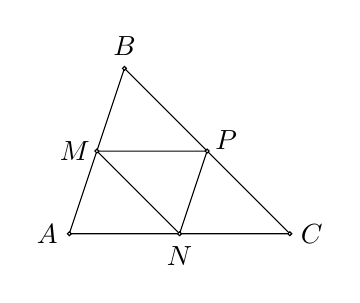
\begin{tikzpicture}[scale=0.7]
        \draw (0,0) coordinate (A)--(1,3)coordinate (B)--(4,0)coordinate (C)--cycle;
        \draw (barycentric cs:A=1,B=1) coordinate (M)--(barycentric cs:A=1,C=1) coordinate (N)--(barycentric cs:B=1,C=1) coordinate (P)--cycle;
        \foreach \p/\q in {A/180,B/90,C/0,M/180,N/-90,P/30}
        \draw[fill=white](\p)circle(1pt)+(\q:.4)node{$\p$};
        \end{tikzpicture}
    }
} 
\end{vd}

\begin{vd}%[Hồng Trường Sơn]%[0H1B2-2]
    Cho hai hình bình hành $ABCD$ và $AB'C'D'$. Chứng minh rằng 
    $$\vec{B'B}+\vec{CC'}+\vec{D'D}=\vec{0}.$$
    \loigiai{
    Do $ABCD$ và $AB'C'D'$ là hai hình bình hành nên 
    $$\heva{&\vec{AB}+\vec{AD}=\vec{AC}\\ &\vec{AB'}+\vec{AD'}=\vec{AC'}} \Leftrightarrow \heva{&\vec{AB}+\vec{AD}-\vec{AC}= \vec{0}\\ &\vec{AB'}+\vec{AD'}-\vec{AC'}=\vec{0}.}$$
        Ta có $\heva{&\vec{B'B}=\vec{AB}-\vec{AB'}\\&\vec{CC'}=\vec{AC'}-\vec{AC}\\&\vec{D'D}=\vec{AD}-\vec{AD'}}$.\\
        $\Rightarrow \vec{B'B}+\vec{CC'}+\vec{D'D}= \left(\vec{AB}+\vec{AD}-\vec{AC}\right)-\left(\vec{AB'}+\vec{AD'}-\vec{AC'}\right)=\vec{0}$.
    }
\end{vd}

\begin{dang}{Xác định vị trí của một điểm nhờ đẳng thức véctơ.}
    Để xác định điểm $M$ thỏa đẳng thức véctơ cho trước, ta thực hiện một trong các hướng sau\\
$\circ$ \textbf{Hướng 1}
\begin{itemize}
    \item [$\bullet$] Biến đổi đẳng thức véctơ đã cho về dạng $\vec{AM}=\vec{v}$, trong đó $A$ cố định và $\vec{v}$ cố định.
    \item [$\bullet$] Khi đó điểm $M$ được xác định
    \begin{itemize}
        \item $\vec{AM},\vec{v}$ cùng hướng.
        \item Độ dài $AM= \left|\vec{v}\right|$.
    \end{itemize}
\end{itemize}
$\circ$ \textbf{Hướng 2}
\begin{itemize}
\item [$\bullet$] Biến đổi đẳng thức véctơ đã cho về dạng $\left\vert \vec{IM}\right\vert=\left\vert \vec{AB}\right\vert$, trong đó $I,A,B$ là các điểm cố định.
\item [$\bullet$] Khi đó điểm $M$ cần tìm thuộc đường tròn tâm $I$, bán kính $AB$.
\end{itemize}
$\circ$ \textbf{Hướng 3}
\begin{itemize}
    \item [$\bullet$] Biến đổi đẳng thức véctơ đã cho về dạng $\left\vert \vec{MA}\right\vert=\left\vert \vec{MB}\right\vert$, trong đó $A,B$ cố định và phân biệt.
    \item [$\bullet$] Khi đó điểm $M$ cần tìm thuộc đường trung trực của đoạn $AB$.
\end{itemize}
\end{dang}
\begin{vd}%[Hồng Trường Sơn]%[0H1B2-3]
    Cho tam giác $ABC$. Tìm điểm $M$ thỏa mãn điều kiện 
    \begin{listEX}[2]
        \item $\vec{BA}+\vec{BC}+\vec{MB}=\vec{0}$.
        \item $\vec{MA}-\vec{MB}+\vec{MC}=\vec{BC}$.
    \end{listEX}
    \loigiai{
    \begin{enumerate}
        \item Ta có 
        \immini{
        \begin{eqnarray*}
            &&\vec{BA}+\vec{BC}+\vec{MB}=\vec{0}\\
            &\Leftrightarrow& \vec{BA}+\vec{MC}=\vec{0}\\
            &\Leftrightarrow& \vec{CM}=\vec{BA}.
        \end{eqnarray*}
        $\Rightarrow$ Điểm $M$ là điểm thứ tư của hình bình hành $ABCM$.}
        {\begin{tikzpicture}[line cap=round,line join=round]
            \tkzInit[xmin=-1,xmax=6,ymin=-1,ymax=3]\tkzClip
            \tkzDefPoints{1/2/A, 0/0/B, 4/0/C}
            \tkzDefPointBy[translation = from B to A](C) \tkzGetPoint{M}
            \tkzDrawPoints[fill=black](A,B,C,M)
            \tkzLabelPoint[ above](A){$A$}
            \tkzLabelPoint[ above](M){$M$}
            \tkzLabelPoint[ below](B){$B$}
            \tkzLabelPoint[ below](C){$C$}
            \tkzDrawSegments(A,B B,C C,A  A,M M,C) 
            \end{tikzpicture}}
        \item Ta có
        \immini{
        \begin{eqnarray*}
            &&\vec{MA}-\vec{MB}+\vec{MC}=\vec{BC}\\
            &\Leftrightarrow& \vec{BA}-\vec{BC}=\vec{CM}\\
            &\Leftrightarrow& \vec{CA}=\vec{CM}.
        \end{eqnarray*}
        $\Rightarrow$ Điểm $M$ trùng với điểm $A$.}
        {\begin{tikzpicture}[line cap=round,line join=round]
            \tkzInit[xmin=-1,xmax=5,ymin=-1,ymax=3]\tkzClip
            \tkzDefPoints{1/2/A, 0/0/B, 4/0/C}
            \tkzDrawPoints[fill=black](A,B,C)
            \tkzLabelPoint[ above](A){$A$}
            \tkzLabelPoint[ below](B){$B$}
            \tkzLabelPoint[ below](C){$C$}
            \tkzDrawSegments(A,B B,C C,A) 
            \end{tikzpicture}}
    \end{enumerate}
    }
\end{vd}

\begin{vd}%[Hồng Trường Sơn]%[0H1B2-3]
    Cho tam giác $ABC$. Gọi $I,K$ lần lượt là trung điểm của các đoạn thẳng $BC, AI$. Tìm điểm $M$ thỏa mãn điều kiện $\vec{BA}+\vec{BI}-\vec{BM}+\vec{AK}+\vec{IC}=\vec{0}$.
    \loigiai{
    \immini{Ta có
    \begin{eqnarray*}
        &&\vec{BA}+\vec{BI}-\vec{BM}+\vec{AK}+\vec{IC}=\vec{0} \\
        &\Leftrightarrow& \vec{BA}+\vec{MI}+\vec{AK}+\vec{IC}=\vec{0}\\
        &\Leftrightarrow& \vec{MC}+\vec{BK}=\vec{0}\\
        &\Leftrightarrow& \vec{CM}=\vec{BK}.
    \end{eqnarray*}
    }
        {\begin{tikzpicture}[line cap=round,line join=round]
            \tkzInit[xmin=-1,xmax=7,ymin=-1,ymax=2.5]\tkzClip
            \tkzDefPoints{1/2/A, 0/0/B, 4/0/C}
            \tkzDefMidPoint(B,C)\tkzGetPoint{I}
            \tkzDefMidPoint(A,I)\tkzGetPoint{K}
            \tkzDefPointBy[translation = from B to K](C) \tkzGetPoint{M}
            \tkzDrawPoints[fill=black](A,B,C,M,I,K)
            \tkzLabelPoint[ above](A){$A$}
            \tkzLabelPoint[ above](M){$M$}
            \tkzLabelPoint[ below](B){$B$}
            \tkzLabelPoint[ below](C){$C$}
            \tkzLabelPoint[ left](K){$K$}
            \tkzLabelPoint[below](I){$I$}
            \tkzDrawSegments(A,B B,C C,A A,I K,M C,M B,K) 
            \end{tikzpicture}}
        \noindent Vậy điểm $M$ là đỉnh thứ tư của hình bình hành $CBKM$.
        }
\end{vd}

\begin{vd}%[Hồng Trường Sơn]%[0H1K2-3]
    Cho  tam giác $ABC$. Tìm điểm $M$ thỏa mãn $\vert\vec{BA}-\vec{BM}\vert =\vert\vec{MA}+\vec{AC}\vert$.
    \loigiai{
    Ta có
    $$\vert\vec{BA}-\vec{BM}\vert =\vert\vec{MA}+\vec{AC}\vert \Leftrightarrow MA=MC.$$
        $\Rightarrow$ Điểm $M$ thuộc đường trung trực của đoạn thẳng $AC$.
    }
\end{vd}
%
\begin{vd}%[Hồng Trường Sơn]%[0H1K2-3]
    Cho tam giác $ABC$. Tìm điểm $M$ thỏa mãn điều kiện $\vert\vec{MA}\vert=\vert\vec{MB}-\vec{MC}\vert$.
    \loigiai{
    \immini{Ta có
    \begin{eqnarray*}
        &&\vert\vec{MA}\vert=\vert\vec{MB}-\vec{MC}\vert\\
        &\Leftrightarrow& \vert \vec{MA}\vert =\vert \vec{CB}\vert\\
        &\Leftrightarrow& MA =CB.
    \end{eqnarray*}
        $\Rightarrow$ Điểm $M$ thuộc đường tròn tâm $A$, bán kính $CB$.}
        {\begin{tikzpicture}[line cap=round,line join=round]
            \tkzInit[xmin=-1,xmax=4,ymin=-1,ymax=3.5]\tkzClip
            \tkzDefPoints{1/1/A, 0/0/B, 2/0/C}
            \tkzDrawPoints[fill=black](A,B,C)
            \tkzLabelPoint[ above](A){$A$}
            \tkzLabelPoint[ below](B){$B$}
            \tkzLabelPoint[ below](C){$C$}
            \tkzDrawSegments(A,B B,C C,A) 
            \tkzDefPointBy[translation = from B to C](A) \tkzGetPoint{M}
            \tkzDrawPoints[fill=black](M)
            \tkzLabelPoint[ right](M){$M$}
            \tkzDrawCircle(A,M)
            \tkzDrawSegments(A,M C,M) 
            \end{tikzpicture}}
    }
\end{vd}

\begin{dang}{Tính độ dài của tổng, hiệu các véctơ}
    Để tính độ dài của các véctơ $\vec{a}+\vec{b}$ và $\vec{a}-\vec{b}$ ta thường thực hiện các bước sau
\begin{enumerate}[Bước 1.]
    \item Dùng các quy tắc véctơ để xác định $\vec{a}+\vec{b}$ và $\vec{a}-\vec{b}$.
        \item Dùng tính chất của hình học phẳng để đưa bài toán tính độ dài véctơ thành bài toán tính độ dài đoạn thẳng trong hình đặc biệt đã biết cách tính.
    \end{enumerate}
\end{dang}

\begin{vd}%[Hồng Trường Sơn]%[0H1B2-5]
    Cần thêm điều kiện gì của hai véctơ $\vec{a}$ và $\vec{b}$ khác $\vec{0}$ để
\begin{listEX}[2]
    \item $\left|\vec{a}+\vec{b}\right|=\left|\vec{a}\right|+\left|\vec{b}\right|$.
    \item $\left|\vec{a}-\vec{b}\right|=\left|\vec{a}\right|-\left|\vec{b}\right|$.
\end{listEX}
\loigiai{
\begin{listEX}
    \item Với hai véctơ $\vec{a}$ và $\vec{b}$ bất kỳ khác $\vec{0}$ ta luôn dựng được $\vec{AB}=\vec{a}$, $\vec{BC}=\vec{b}$.\\
    Khi đó, ta có 
    $$\left|\vec{a}+\vec{b}\right|=\left|\vec{AB}+\vec{BC}\right|=\left|\vec{AC}\right|=AC\leq AB+BC=\left|\vec{a}\right|+\left|\vec{b}\right|.$$ 
    Dấu bằng xảy ra khi $B$ nằm giữa $A$ và $C$ hay $\vec{AB}$, $\vec{BC}$ cùng hướng.\\
    Vậy $\left|\vec{a}+\vec{b}\right|=\left|\vec{a}\right|+\left|\vec{b}\right|$ khi $\vec{a}$ và $\vec{b}$ cùng hướng.
    \item Dựng $\vec{OA}=\vec{a}$, $\vec{OB}=\vec{b}$. Khi đó, ta có 
    $$\left|\vec{a}-\vec{b}\right|=\left|\vec{OA}-\vec{OB}\right|=\left|\vec{BA}\right|\geq OA-OB=\left|\vec{a}\right|-\left|\vec{b}\right|.$$
    Dấu bắng xảy ra khi $B$ nằm giữa $O$ và $A$ hay $\vec{OA}$ và $\vec{OB}$ cùng hướng. 
\end{listEX}
\begin{nx}
    \begin{listEX}[2]
    \item $\left|\vec{a}+\vec{b}\right|\leq \left|\vec{a}\right|+\left|\vec{b}\right|$.
    \item $\left|\vec{a}-\vec{b}\right|\geq \left|\vec{a}\right|-\left|\vec{b}\right|$.
    \end{listEX}
Dấu đẳng thức xảy ra khi và chỉ khi $\vec{a}$ và $\vec{b}$ cùng hướng.
\end{nx}
}
\end{vd}

\begin{vd}%[Hồng Trường Sơn]%[0H1B2-5]
Cho tam giác $ABC$ vuông tại $A$. $AB=2a$, $AC=a$. Tính độ dài các véctơ 
\begin{listEX}[2]
    \item $\vec{AB}+\vec{AC}$.
    \item $\vec{AB}-\vec{AC}$.
\end{listEX}
\loigiai{
\immini{
    \begin{listEX}
        \item Dựng hình chữ nhật $ABDC$. Ta có
        $$\vec{AB}+\vec{AC}=\vec{AD}.$$
        Suy ra $\left|\vec{AB}+\vec{AC}\right|=AD=BC=\sqrt{BA^2+AC^2}=a\sqrt{5}$.
        \item Ta có $\vec{AB}-\vec{AC}=\vec{CB}$.\\ 
        Suy ra $\left|\vec{AB}+\vec{AC}\right|=CB=a\sqrt{5}$.
    \end{listEX}
}
{
\begin{tikzpicture}[line join = round, line cap = round,>=stealth,thick,font=\footnotesize,scale=1]
\draw (90:4)coordinate(B)--(0,0)coordinate(A)--(0:2)coordinate(C)--($(B)+(C)-(A)$)coordinate(D)--(B)--(C) pic[fill=blue!50,angle radius=2mm]{right angle=B--A--C};
\path (A)--(B) node[left,midway]{$2a$};
\path (A)--(C) node[above,midway]{$a$};
\foreach \p/\g in {A/180,B/90,C/0,D/60}
{\path (\p)+(\g:3mm) node{$\p$};
    \fill (\p) circle(1pt);};
\end{tikzpicture}
}
}
\end{vd}

\begin{vd}%[Hồng Trường Sơn]%[0H1B2-5]
    Cho tam giác đều $ABC$ có cạnh bằng $a$. Tính độ dài của các véctơ sau 
\begin{listEX}[3]
    \item $\vec{AB}-\vec{AC}$.
    \item $\vec{AB}+\vec{AC}$.
    \item $\vec{AB}+\vec{CB}$.
\end{listEX}
    \loigiai{
        \immini{
            \begin{listEX}
                \item Ta có $\left|\vec{AB}-\vec{AC}\right|=CB=a$.
                \item Dựng hình bình hành $ABEC$, ta có 
                \begin{eqnarray*}
                    \left|\vec{AB}+\vec{AC}\right|&=&\left|\vec{AE}\right|=AE\\
                    &=&2\cdot\dfrac{a\sqrt{3}}{2}=a\sqrt{3}.
                \end{eqnarray*}
                \item Lấy $C'$ sao cho $B$ là trung điểm $CC'$. 
                \end{listEX}
        }{\begin{tikzpicture}[>=stealth,scale=0.6]
            \def \a{4};
            \path[draw] (0,0)coordinate(B)--+(\a,0)coordinate(C)--(60:\a)coordinate(A)--(B)--(180:\a)coordinate(D)node[below]{$C'$} (D)--(A)--($(B)+(C)-(A)$) coordinate(E)--(B)--($(D)!(B)!(A)$)coordinate(H) (E)--(C);
            \foreach \p/\g in {A/90,B/-120,C/0,E/-90,H/120}
            {\path (\p)+(\g:3mm) node{$\p$};
                \fill (\p) circle(1pt);};
            \end{tikzpicture}}
            \noindent Khi đó $\vec{CB}=\vec{BC'}$, suy ra $\vec{AB}+ \vec{CB}= \vec{AB}+ \vec{BC'} = \vec{AC'} \Rightarrow \left|\vec{AB}+ \vec{CB} \right| = \left|\vec{AC'} \right|$.\\
            Trong $\triangle ABC'$ cân tại $B$, kẻ $BH \perp AC'$, ta có $\triangle BHA$ có $AB=a$, $\widehat{HBA} = 60 ^ \circ$.\\ 
                Do đó $AH= AB \cdot \sin \widehat{HBA} =  \dfrac{a \sqrt{3}}{2}$ suy ra $AC'  = a\sqrt{3}$.\\
                Vậy độ dài của vectơ $\vec{AB}+ \vec{CB}$ là $a\sqrt{3}$.
        }
\end{vd}

\begin{vd}%[Hồng Trường Sơn]%[0H1B2-5]
    Cho hình vuông $ABCD$ cạnh $a$. Tính $\left|\vec{AB} - \vec{AC}\right|$,  $\left|\vec{AB} + \vec{AD}\right|$ theo $a$.
    \loigiai{
        \immini{
            Ta có 
            \begin{itemize}
                \item $\vec{AB} - \vec{AC} = \vec{CB}$.\\
                Do đó $\left|\vec{AB} - \vec{AC}\right| = \left|\vec{CB}\right| = CB = a$.
                \item $\left|\vec{AB} + \vec{AD}\right|=\left|\vec{AC}\right|=AC=a\sqrt{2}$.
            \end{itemize}
        }
        {\begin{tikzpicture}[>=stealth,scale=0.6,x=1cm,y=1cm]
            \def \a{4};
            \path[draw] (0,0)coordinate(A)--++(\a,0)coordinate(B)--++(90:\a)coordinate(C)--(90:\a)coordinate(D)--cycle;
            \foreach \p/\g in {A/-90,B/-90,C/90,D/90}
            {\path (\p)+(\g:3mm) node{$\p$};
                \fill (\p) circle(1pt);};
            \end{tikzpicture}
        }
    }
\end{vd}
\begin{vd}%[Hồng Trường Sơn]%[0H1B2-5]
    Cho hình bình hành $ABCD$ tâm $O$. Chứng minh rằng
    \begin{listEX}[1]
        \item $\left|\vec{AB} + \vec{AD}\right|=AC$.
        \item Nếu $\left|\vec{AB} + \vec{AD}\right|=\left|\vec{CB}- \vec{CD}\right|$ thì $ABCD$ là hình chữ nhật.
    \end{listEX}
    \loigiai
    {
    \immini
    {
        \begin{listEX}[1]
        \item $\left|\vec{AB} + \vec{AD}\right|=\left|\vec{AC}\right|=AC$.
        \item Ta có $\left|\vec{AB} + \vec{AD}\right|=AC$; $\left|\vec{CB}- \vec{CD}\right|=BD$.\\ 
        Nếu $AC=BD$ bằng nhau thì hình hình hành $ABCD$ là hình chữ nhật.
    \end{listEX}
    }
    {
    \begin{tikzpicture}[>=stealth,scale=0.6,x=1cm,y=1cm]
    \def \a{4};
    \path[draw] (80:\a) coordinate(D)--(0,0)coordinate(A)--++(\a,0)coordinate(B)--($(B)+(D)-(A)$)coordinate(C)--cycle;
    \foreach \p/\g in {A/-90,B/-90,C/90,D/90}
    {\path (\p)+(\g:3mm) node{$\p$};
        \fill (\p) circle(1pt);};
    \end{tikzpicture}
    }
    }
\end{vd}
\begin{vd}%[Hồng Trường Sơn]%[0H1K2-5]
    Cho hai lực $\vec{F_1}=\vec{MA}$; $\vec{F_2}=\vec{MB}$ cùng tác động vào một vật tại điểm $M$. Cường độ hai lực $\vec{F_1};\vec{F_2}$ lần lượt là $300N$ và $400N.$ Tìm cường độ lực tổng hợp tác động vào vật, biết  $\widehat{AMB}=90^{\circ}$.
    \loigiai{ 
    \immini
    {
    Áp dụng định lí Pitago ta có  cường độ của lực tổng hợp 
    $$|\vec{F}|=\sqrt{|\vec{F_1}|^2+|\vec{F_2}|^2}=500N.$$
    }
    {
    \begin{tikzpicture}[>=stealth,scale=0.8]
    \def \a{3};
    \path[draw] (0,0)coordinate(M) (45:\a) coordinate(A) (-45:\a)coordinate(B)--($(A)+(B)-(M)$)coordinate(C)--(A);
    \path (M)--(C) node[above,midway]{\footnotesize $\vec{F}$};
    \path (M)--(A) node[above,midway]{\footnotesize $\vec{F}_1$};
    \path (M)--(B) node[left,midway]{\footnotesize $\vec{F}_2$};
    \foreach \p/\g in {M/A,M/B,M/C}\draw[->] (\p)--(\g);
    \foreach \p/\g in {A/90,B/-90,C/0,M/-120}
    {\path (\p)+(\g:5mm) node{$\p$};
        \fill (\p) circle(1pt);};
    \end{tikzpicture}
    }
    }
\end{vd}


\subsection{Bài tập tự luận}
\begin{bt}%[0H1B2-2]
	Cho bốn điểm $A,B,C,D$. Chứng minh rằng
\begin{multicols}{2}
	\begin{enumerate}
		\item $\overrightarrow{AB}+\overrightarrow{BC}+\overrightarrow{CD}+\overrightarrow{DA}=\overrightarrow{0}$.
		\item $\overrightarrow{AC}-\overrightarrow{AD}=\overrightarrow{BC}-\overrightarrow{BD}$.
	\end{enumerate}
\end{multicols}
	\loigiai
	{
	\begin{enumerate}
		\item 	Ta có
\allowdisplaybreaks
\begin{eqnarray*}
\overrightarrow{AB}+\overrightarrow{BC}+\overrightarrow{CD}+\overrightarrow{DA}
&=&(\overrightarrow{AB}+\overrightarrow{BC})+(\overrightarrow{CD}+\overrightarrow{DA})\\
&=&\overrightarrow{AC}+\overrightarrow{CA}\\
&=&\overrightarrow{0}
\end{eqnarray*}
\item
$ \heva{& \overrightarrow{AD} -\overrightarrow{AD}=\overrightarrow{DC} \\ & \overrightarrow{BC}-\overrightarrow{BD}=\overrightarrow{DC}}\Rightarrow \overrightarrow{AC}-\overrightarrow{AD}=\overrightarrow{BC}-\overrightarrow{BD}$.
	\end{enumerate}

	}
\end{bt}
\begin{bt}%[0H1B2-3]
	Cho hình bình hành $ABCD$. Hãy tìm điểm $M$ để $\overrightarrow{BM}=\overrightarrow{AB}+\overrightarrow{AD}$. Tìm mối quan hệ giữa hai vectơ $\overrightarrow{CD}$ và $\overrightarrow{CM}$.
	\loigiai
	{
		\immini
		{
			Vì $ABCD$ là hình bình hành nên $\overrightarrow{AB}+\overrightarrow{AD}=\overrightarrow{AC}$.\\
			Do đó $\overrightarrow{BM}=\overrightarrow{AC}$, suy ra $M$ là đỉnh  của hình bình hành $ABMC$.\\
			Vậy $\overrightarrow{CM}=\overrightarrow{AB}=-\overrightarrow{CD}$.
			
		}
		{
			\begin{tikzpicture}[line cap=round,line join=round]
				\tkzInit[xmin=-1,xmax=5.5,ymin=-3,ymax=3]\tkzClip
				\tkzDefPoints{1/2/A, 0/0/B, 4/0/C}
				\tkzDefPointBy[translation = from B to A](C) \tkzGetPoint{D}
					\tkzDefPointBy[translation = from A to C](B) \tkzGetPoint{M}
				\tkzDrawPoints[fill=black](A,B,C,D,M)
				\tkzLabelPoint[ above](A){$A$}
				\tkzLabelPoint[ above](D){$D$}
				\tkzLabelPoint[ below](B){$B$}
				\tkzLabelPoint[ below](C){$C$}
				\tkzLabelPoint[ below](M){$M$}
				\tkzDrawSegments(A,B B,C C,A  A,D D,C B,M C,M) 
			\end{tikzpicture}
		}

	}
\end{bt}
\begin{bt}%[0H1B2-5]
	Cho tam giác đều $ABC$ có cạnh bằng $a$. Tính độ dài các vectơ $\overrightarrow{AB}-\overrightarrow{AC}$, $\overrightarrow{AB}+\overrightarrow{AC}$.
	\loigiai{
		\immini{
			$\bullet$ Ta có $\left|\vec{AB}-\vec{AC}\right|=CB=a$.\\
			$\bullet$ Gọi $E$ là trung điểm của $BC$ ta có 
				\begin{eqnarray*}
					\left|\vec{AB}+\vec{AC}\right|&=&\left|2\vec{AE}\right|=2AE\\
					&=&2\cdot\dfrac{a\sqrt{3}}{2}=a\sqrt{3}.
				\end{eqnarray*}
		}
	{
		\begin{tikzpicture}[>=stealth,line join=round,line cap=round,font=\footnotesize,scale=1]
	\tkzDefPoints{0/0/B, 3/0/C}
		\tkzDrawEquilateral(B,C) 
		\tkzDefPointBy[rotation = center B angle 60](C) \tkzGetPoint{A}
		\tkzDefMidPoint(B,C) \tkzGetPoint{E}
		\tkzDrawSegments(A,E) 
		\tkzDrawPoints[fill=black](A,B,C,E)
		\tkzLabelPoint[ above](A){$A$}
	\tkzLabelPoint[ right](C){$C$}
	\tkzLabelPoint[ left](B){$B$}
	\tkzLabelPoint[ below](E){$E$}	
	\end{tikzpicture} 
		
	}

	}
\end{bt}
\begin{bt}%[0H1T2-5]
\immini
{
Hình $4.19$ biểu diễn hai lực $\overrightarrow{F_1}, \overrightarrow{F_2}$ cùng tác động lên một vật, cho $|\overrightarrow{F_1}|=3\,N$, $|\overrightarrow{F_2}|=2\, N$. Tính độ lớn của hợp lực $\overrightarrow{F_1}+\overrightarrow{F_2}$.
}
{
		\begin{tikzpicture}[>=stealth,line join=round,line cap=round,font=\footnotesize,scale=1]
		\tkzDefPoints{0/0/O,-1/2/A,3/0/B}
\draw[->](O) -> (A);
\draw[->](O) -> (B);	
	\draw pic[draw,blue,fill=green!50,opacity=.5,angle radius=3mm] {angle = B--O--A}; 
\tkzLabelAngles[pos=0.5,rotate=-25](B,O,A){$120^\circ$}
	\node at (1,-1){Hình 4.19};
	\tkzLabelLine[pos=.5,below,blue](O,B){$\overrightarrow{F_2}$}
	\tkzLabelLine[pos=.5,left,blue](O,A){$\overrightarrow{F_1}$}
		
	\end{tikzpicture}
}	
	
	\loigiai
	{
	\immini
	{
		Dựng hình bình hành $ABCD$ như hình. \\
		Ta có $|\overrightarrow{F_1}+\overrightarrow{F_2}|=|\overrightarrow{AC}|=AC$.\\
		Trong $\triangle ABC$ ta có
		\begin{eqnarray*}
				AC&=&\sqrt{AB^2+BC^2-2AB\cdot BC\cdot \cos 60^\circ}\\
					&=&\sqrt{2^2+3^2-2\cdot 2\cdot 3\cdot \dfrac{1}{2}}\\
					&=&\sqrt{7}.
		\end{eqnarray*}
	Vậy $|\overrightarrow{F_1}+\overrightarrow{F_2}|=7\,\text{N}$.
	}
	{
		\begin{tikzpicture}[>=stealth,line join=round,line cap=round,font=\footnotesize,scale=1]
		\tkzDefPoints{0/0/A,-1/2/B,3/0/D}
		\draw[->](A) -> (B);
		\draw[->](A) -> (D);	
		\draw pic[draw,blue,fill=green!50,opacity=.5,angle radius=3mm] {angle = D--A--B}; 
		\tkzLabelAngles[pos=0.5,rotate=-25](B,A,D){$120^\circ$}
		\node at (1,-1){Hình 4.19};
			\tkzDefPointBy[translation = from A to D](B) \tkzGetPoint{C}
		\tkzLabelLine[pos=.5,left,blue](A,B){$\overrightarrow{F_2}$}
		\tkzLabelLine[pos=.5,below,blue](A,D){$\overrightarrow{F_1}$}
			\tkzLabelPoint[left](B){$B$}
		\tkzLabelPoint[ right](D){$D$}
			\tkzLabelPoint[ right](C){$C$}
		\tkzLabelPoint[ below](A){$A$}	
			\tkzDrawSegments(A,C C,B D,C)
	\end{tikzpicture}
	}
	}
\end{bt}
\begin{bt}%[0H1T2-5]
	\immini{
	Hai con tàu cùng xuất phát từ bờ bên này để sang bờ bên kia của dòng sông với vận tốc không đổi và có độ lớn bằng nhau. Hai tàu luôn được giữ lái sao cho chúng tạo với bờ cùng một góc nhọn nhưng một tàu hướng xuống hạ lưu, một tàu hướng lên thượng nguồn (hình bên). Vận tốc dòng nước là đáng kể, các yếu tố bên ngoài khác không ảnh hưởng đến vận tốc của các tàu. Hỏi tàu nào sang bờ bên kia trước?}
{	\begin{tikzpicture}[line join=round, line cap=round,>=stealth,scale=.8]
		\foreach \x in {1,2,3}
		\foreach \y in {0,1,2,3,4,5}
		\draw(0.25+\y,\x-0.25)--(\y,\x-0.25) ;
		\foreach \x in {1,2,3}
		\foreach \y in {0,1,2,3,4,5}
		\draw(-0.25+\y,\x-0.75)--(\y,\x-0.75) ;
		\tkzDefPoints{3/0/A_1,6/3/B_1,3.5/3/C_1,2/0/A_2, -1/3/B_2,-3/3/C_2, 6/0/H_1,-1/0/H_2}
		\coordinate (M_1) at ($(A_1)!0.4!(B_1)$);
		\coordinate (N_1) at ($(A_1)!0.4!(C_1)$);
		\coordinate (M_2) at ($(A_2)!0.4!(B_2)$);
		\coordinate (N_2) at ($(A_2)!0.4!(C_2)$);
		\draw[thick,blue] (0,3)--(5,3);
		\draw[thick,blue] (0,0)--(5,0);
		\tkzDefMidPoint(A,B) \tkzGetPoint{40}
		\tkzDefMidPoint(A,C) \tkzGetPoint{30} 
		\tkzDrawPoints[fill=black](A_1,A_2)
		\draw[->,thick,blue](A_1) -> (M_1);% Vẽ trục số
		\draw[->,thick,red](A_2) -> (M_2);% Vẽ trục số
		\tkzLabelAngles[pos=0.5,rotate=30](B_1,A_1,H_1 B_2,A_2,H_2){$\alpha$}
		\tkzMarkAngles[size=1cm,arc=l](H_1,A_1,B_1 B_2,A_2,H_2)
		\tkzLabelPoint[ below](A_1){$A_1$}	
		\tkzLabelPoint[ below](A_2){$A_2$}
	\end{tikzpicture}
}
	\loigiai
	{
\begin{center}
\begin{tikzpicture}[line join=round, line cap=round,>=stealth,scale=1]
	\foreach \x in {1,2,3}
	\foreach \y in {-2,-1,0,1,2,3,4,5,6}
	\draw(0.25+\y,\x-0.25)--(\y,\x-0.25) ;
	\foreach \x in {1,2,3}
	\foreach \y in {-2,-1,0,1,2,3,4,5,6}
	\draw(-0.25+\y,\x-0.75)--(\y,\x-0.75) ;
	\tkzDefPoints{3/0/A_1,6/3/B_1,3.5/3/C_1,2/0/A_2, -1/3/B_2,-3.5/3/C_2, 6/0/H_1,-1/0/H_2}
	\coordinate (M_1) at ($(A_1)!0.4!(B_1)$);
		\coordinate (N_1) at ($(A_1)!0.4!(C_1)$);
			\coordinate (M_2) at ($(A_2)!0.4!(B_2)$);
		\coordinate (N_2) at ($(A_2)!0.4!(C_2)$);
	\draw[thick,blue] (-2.5,3)--(7,3);
	\draw[thick,blue] (-2.5,0)--(7,0);
	\tkzDefMidPoint(A,B) \tkzGetPoint{40}
	\tkzDefMidPoint(A,C) \tkzGetPoint{30} 
	\tkzDrawPoints[fill=black](A_1,B_1,A_2,B_2,H_1,H_2)
	\tkzDrawSegments(A_1,B_1 A_2,B_2  B_1,H_1 B_2,H_2)
	\draw[->,thick,blue](A_1) -> (N_1);% Vẽ trục số
	\draw[->,thick,blue](A_1) -> (M_1);% Vẽ trục số
	\draw[->,thick,blue](M_1) -> (N_1);% Vẽ trục số
	\draw[->,thick,red](A_2) -> (N_2);% Vẽ trục số
	\draw[->,thick,red](A_2) -> (M_2);% Vẽ trục số
	\draw[->,thick,red](M_2) -> (N_2);% Vẽ trục số
		\draw[->,thick,red](5,2.25) -> (0,2.25);% Vẽ trục số
		\node at (2.5,2.45){$\text{hướng dòng nước chảy}$};
\tkzLabelLine[pos=0.5,right,blue](H_1,B_1){$d$}
	\tkzLabelLine[pos=0.5,left,blue](H_2,B_2){$d$}
\tkzLabelAngles[pos=0.5,rotate=30](B_1,A_1,H_1 B_2,A_2,H_2){$\alpha$}
\tkzMarkAngles[size=1cm,arc=l](H_1,A_1,B_1 B_2,A_2,H_2)
	\tkzLabelPoint[above](B_1){$B_1$}
\tkzLabelPoint[ above](B_2){$B_2$}
\tkzLabelPoint[ below](A_1){$A_1$}	
\tkzLabelPoint[ below](A_2){$A_2$}
\tkzLabelPoint[ above right](M_2){$M_2$}
\tkzLabelPoint[ below](H_1){$H_1$}
\tkzLabelPoint[below](H_2){$H_2$}
\tkzLabelPoint[right](M_1){$M_1$}
\tkzLabelPoint[above](N_1){$N_1$}
\tkzLabelPoint[above left](N_2){$N_2$}
\end{tikzpicture}
\end{center}
Gọi\\
$\cdot$ $B_1, B_2$ lần lượt là vị trí của tàu $A_1, A_2$ cập bờ bên kia.\\
$\cdot$ $\overrightarrow{v_1}=\overrightarrow{A_1M_1}$ và $\overrightarrow{v_2}=\overrightarrow{A_2M_2}$  là vận tốc riêng của hai tàu $A_1$ , $A_2$.Theo giả thiết $|\overrightarrow{v_1}|=|\overrightarrow{v_2}|=v$.\\
$\cdot$ $\overrightarrow{v_n}=\overrightarrow{M_1N_1}=\overrightarrow{M_2N_2}$ là vận tốc của dòng nước.\\
$\cdot$$\overrightarrow{v_{A_1}}=\overrightarrow{A_1N_1}$ và $\overrightarrow{v_{A_2}}=\overrightarrow{A_2N_2}$ lần lượt là vận tốc thực tế của tàu $A_1$ và $A_2$.\\
$\cdot$ $d=B_1H_1=B_2H_2$ là khoảng cách giữa hai bờ sông.\\
Ta có\\
$\cdot$ $v_{A_1}=\sqrt{v^2+v_n^2-2vv_n\cdot \cos \widehat {A_1M_1N_1} }=\sqrt{v^2+v_n^2-2vv_n\cdot \cos \alpha}$\\
$\cdot$  $v_{A_2}=\sqrt{v^2+v_n^2-2vv_n\cdot \cos \widehat {A_2M_2N_2} }=\sqrt{v^2+v_n^2+2vv_n\cdot \cos \alpha}$ (vì $\widehat {A_2M_2N_2}=180^\circ -\alpha $).\\
Suy tra $v_{A_1}<v_{A_2}$. Mà $\sin \alpha =\dfrac{d}{A_1B_1}=\dfrac{d}{A_2B_2}\Rightarrow A_1B_1=A_2B_2=s$. \\Do đó
thời gian để tàu $A_1,A_2$ sang bờ bên kia  lần lượt là $t_1=\dfrac{s}{v_{A_1}}>t_2=\dfrac{s}{v_{A_2}}$ (vì $v_{A_1}<v_{A_2}$).\\
Vậy tàu $A_2$ sẽ sang bờ bên kia trước.
}
\end{bt}
\Closesolutionfile{ans}



\subsection{Bài tập}
\Opensolutionfile{ans}
\setcounter{ex}{0}
\begin{ex}%[0H1Y2-1]
Cho ba điểm $M$, $N$, $P$. Vectơ $\vec{u}=\overrightarrow{NP}+\overrightarrow{MN}$ bằng vectơ nào sau đây?
\choice
{$\overrightarrow{PN}$}
{$\overrightarrow{PM}$}
{\True $\overrightarrow{MP}$}
{$\overrightarrow{NM}$}
\loigiai{
Ta có
$$
\overrightarrow{NP}+\overrightarrow{MN}=\overrightarrow{MN}+\overrightarrow{NP}=\overrightarrow{MP}.
$$
}
\end{ex}

\begin{ex}%[0H1Y2-1]
Cho ba điểm $D$, $E$, $G$. Vectơ $\overrightarrow{v}=\overrightarrow{DE}+(-\overrightarrow{DG})$ bằng vectơ nào sau đây?
\choice
{$\overrightarrow{EG}$}
{\True$\overrightarrow{GE}$}
{$\overrightarrow{GD}$}
{$\overrightarrow{ED}$}
\loigiai{
Ta có
$$
\overrightarrow{DE}+(-\overrightarrow{DG}) = \overrightarrow{DE}+\overrightarrow{GD}=\overrightarrow{GD}+\overrightarrow{DE} = \overrightarrow{GE}.
$$
}
\end{ex}

\begin{ex}%[0H1B2-1]
Cho hình bình hành $ABCD$ có tâm $O$. Các khẳng định sau là đúng hay sai?
\begin{listEX}
\item $\left|\overrightarrow{AB}+\overrightarrow{AD} \right|=\left|\overrightarrow{AC}\right|$.
\item $\overrightarrow{AB}+\overrightarrow{BD}=\overrightarrow{CB}$.
\item $\overrightarrow{OA}+\overrightarrow{OB}=\overrightarrow{OC}+\overrightarrow{OD}$.
\end{listEX}
\loigiai{
\begin{center}
\begin{tikzpicture}
\path
(0,0) coordinate (A)
(-130:3) coordinate (D)
(0:5) coordinate (B)
($(B)!0.5!(D)$) coordinate (O)
($(B)+(D)-(A)$) coordinate (C);
\draw (A)--(B)--(C)--(D)--cycle (A)--(C) (B)--(D);
\foreach \x/\g in {A/150,B/0,C/-30,D/180,O/90}
\fill (\x) circle (1pt) +(\g:3mm) node {$\x$};
\end{tikzpicture}
\end{center}
\begin{listEX}
\item Ta có
$$
\left|\overrightarrow{AB}+\overrightarrow{AD} \right|=\left|\overrightarrow{AB}+\overrightarrow{BC} \right| = \left| \overrightarrow{AC}\right|.
$$
Đây là một khẳng định đúng.
\item Ta có
$$
\overrightarrow{AB}+\overrightarrow{BD}=\overrightarrow{AD}=\overrightarrow{BC}.
$$
Đây là khẳng định sai.
\item Ta có
$$
\overrightarrow{OA}+\overrightarrow{OB}=-\overrightarrow{OC}-\overrightarrow{OD}=-(\overrightarrow{OC}+\overrightarrow{OD}).
$$
Đây là khẳng định sai.
\end{listEX}
}
\end{ex}

\begin{ex}%[0H1Y1-2]
Cho đường tròn tâm $O$. Giả sử $A$ và $B$ là hai điểm nằm trên đường tròn. Tìm điều kiện cần và đủ để hai vectơ $\overrightarrow{OA}$ và $\overrightarrow{OB}$ đối nhau.
\loigiai{
Hai vectơ $\overrightarrow{OA}$ và $\overrightarrow{OB}$ đối nhau
$$
\Leftrightarrow \overrightarrow{OA}=-\overrightarrow{OB} \Leftrightarrow \overrightarrow{OA}=\overrightarrow{BO}.
$$
Suy ra $O$ là trung điểm của $AB$. Hay $AB$ là đường kính của đường tròn $(O)$.
}
\end{ex}

\begin{ex}%[0H1Y2-2]
Cho $ABCD$ là hình bình hành. Chứng minh $\overrightarrow{MB}-\overrightarrow{MA}=\overrightarrow{MC}-\overrightarrow{MD}$ với mỗi điểm $M$ trong mặt phẳng.
\loigiai{
\begin{center}
	\begin{tikzpicture}
		\path
		(0,0) coordinate (A)
		(-130:3) coordinate (D)
		(0:5) coordinate (B)
		($(B)+(D)-(A)$) coordinate (C);
		\draw (A)--(B)--(C)--(D)--cycle;
		\foreach \x/\g in {A/150,B/0,C/-30,D/180}
		\fill (\x) circle (1pt) +(\g:3mm) node {$\x$};
	\end{tikzpicture}
\end{center}	
Ta có
$$
\begin{array}{ccccc}
 & \overrightarrow{MB}-\overrightarrow{MA}&=&\overrightarrow{MC}-\overrightarrow{MD}&\\
 \Leftrightarrow& \overrightarrow{AB} &=& \overrightarrow{DC}& (\text{đúng}).
\end{array}
$$
}
\end{ex}

\begin{ex}%[0H1B2-5]
Cho hình vuông $ABCD$ có cạnh $a$. Tính độ dài của các vectơ sau
\begin{listEX}
\item $\overrightarrow{DA}+\overrightarrow{DC}$.
\item $\overrightarrow{AB}-\overrightarrow{AD}$.
\item $\overrightarrow{OA}+\overrightarrow{OB}$ với $O$ là giao điểm của $AC$ và $BD$.
\end{listEX}
\begin{center}
\begin{tikzpicture}[smooth, line join=round, line cap = round, font=\scriptsize]
\path 
(0,0) coordinate (A)
(90:3) coordinate (B)
(0:3) coordinate (D)
($(B)+(D)-(A)$) coordinate (C)
($(A)!0.5!(C)$) coordinate (O)
($(A)+(B)-(O)$) coordinate (E);
\draw (A)--(B)--(C)--(D)--(A)--(C) (B)--(D) (A)--(E)--(B);
\foreach \x/\g in {A/180,B/180,C/0,D/0,O/-90,E/180} 
\fill (\x) circle (1pt) + (\g:3mm) node {$\x$};
\end{tikzpicture}
\end{center}
\loigiai{
\begin{listEX}
\item Ta có $\left|\overrightarrow{DA}+\overrightarrow{DC} \right|=\left| \overrightarrow{DB}\right|=BD = a\sqrt{2}$.
\item Ta có $\left|\overrightarrow{AB}-\overrightarrow{AD}\right|=\left| \overrightarrow{DB}\right|=BD = a\sqrt{2}$.
\item Ta dựng $\overrightarrow{BE}=\overrightarrow{OA}$, khi đó
$$\left|\overrightarrow{OA}+\overrightarrow{OB}\right|=\left| \overrightarrow{OB}+\overrightarrow{BE}\right|=\left|\overrightarrow{OE} \right|=OE = AD=a.$$
\end{listEX}
}
\end{ex}

\begin{ex}%[0H1K2-1]
Cho ba lực $\overrightarrow{F_1}=\overrightarrow{OA}$, $\overrightarrow{F_2}=\overrightarrow{OB}$ và $\overrightarrow{F_3}=\overrightarrow{OC}$ cùng tác động vào vật tại điểm $O$ và vật đứng yên. Cho biết độ lớn của $\overrightarrow{F_1}$ và $\overrightarrow{F_2}$ đều là $120$ N và $\widehat{AOB}=120^\circ$. Tìm độ lớn và hướng của lực $\overrightarrow{F_3}$.
\loigiai{
\begin{center}
\begin{tikzpicture}[smooth, line join=round, line cap = round, font=\scriptsize,>=latex]
\path 
(0,0) coordinate (O)
(180:4) coordinate (F)
(0:4) coordinate (C)
(120:4) coordinate (A)
(-120:4) coordinate (B);
\draw [->] (O)--(A);
\draw [->] (O)--(B);
\draw [->] (O)--(C);
\draw [dashed,->] (O)--(F);
\draw (A)--(F)--(B);
\draw pic[draw,angle radius=3mm] {angle = A--O--B};
\foreach \x/\g in {O/45,A/90,B/-90,C/-90,F/180}
\fill (\x) circle (0.1pt) + (\g:3mm) node {$\x$};
\end{tikzpicture}
\end{center}
Gọi $F$ thỏa mãn $\overrightarrow{BF}=\overrightarrow{OA}$. Khi đó
$\overrightarrow{OB}+\overrightarrow{OA}=\overrightarrow{OB}+\overrightarrow{BF}=\overrightarrow{OF}$.\\
Để vật cân bằng
\begin{eqnarray*}
\Leftrightarrow& \overrightarrow{OA}+\overrightarrow{OB}+\overrightarrow{OC}&=\overrightarrow{0}\\
\Leftrightarrow &\overrightarrow{OF}+\overrightarrow{OC}&=\overrightarrow{0}
\end{eqnarray*}
Suy ra vectơ $\overrightarrow{OC}=-\overrightarrow{OF}$ nên hai vectơ này ngược hướng và có cùng độ lớn.\\
Khi đó lực $\overrightarrow{F_3}=\left| \overrightarrow{OC}\right|=\left|\overrightarrow{OF} \right|=OF$.\\
Mà tứ giác $OAFB$ là hình thoi có $\widehat{AOB}=120^\circ$ nên $\widehat{AOF}=60^\circ$.\\
Suy ra tam giác $AOF$ đều nên $OF=OA$.\\
Suy ra độ lớn của $\overrightarrow{F_3}=120$ N.
}
\end{ex}

\begin{ex}%[0H1K2-1]
Một dòng sông chảy từ phía bắc xuống phía nam với vận tốc là $10$ km/h. Một chiếc canô chuyển động từ phía đông sang tây với vận tốc $40$ km/h so với mặt nước. Tìm vận tốc của canô so với bờ sông.
\loigiai{
\begin{center}
\begin{tikzpicture}[smooth, line join=round, line cap=round, font=\scriptsize,scale=0.7,>=stealth]
\draw (0,0) -- (0,10) (6,0)--(6,10);
\draw[red,thick,->] (0,6) node[left]{$A$}--(0,4) node[left] {$B$};
\draw[blue,thick,->] (6,6) node[right]{$C$}--(0,4);
\draw[thick,->] (6,6)--(0,6);
\draw (3,6) node[above] {$\vec{v_1}$} (0,5) node[left] {$\vec{v_2}$} (3,5) node[below] {$\vec{v_{12}}$};
\end{tikzpicture}	
\end{center}
Gọi $\overrightarrow{CB}$ là vận tốc của canô, $\overrightarrow{CA}$ là vận tốc của canô theo phương vuông góc với bờ sông và $\overrightarrow{AB}$ là vận tốc của dòng nước. Ta có
$$
\overrightarrow{CB}=\overrightarrow{CA}+\overrightarrow{AB} \Leftrightarrow \overrightarrow{CA}=\overrightarrow{CB}-\overrightarrow{AB}
$$
Khi đó
$$
|\overrightarrow{CA}|=\sqrt{\overrightarrow{CB}^2-\overrightarrow{AB}^2}=\sqrt{40^2-10^2}=10\sqrt{15}.
$$
Vận tốc của canô là $10\sqrt{15}$ km/h.
}
\end{ex}
\Closesolutionfile{ans}

\subsection{Bài tập}
\subsubsection{Bài tập tự luận}
\begin{bt}%[0H1B2-2]
	Cho tứ giác lồi $ABCD$. Gọi $I$, $J$ lần lượt là trung điểm của hai đường chéo $AC$, $BD$.
	\begin{listEX}[1]
		\item Chứng minh rằng $\overrightarrow{AB} + \overrightarrow{CD} = 2\overrightarrow{IJ}$.
		\item Chứng minh rằng $\overrightarrow{AB} + \overrightarrow{AD} + \overrightarrow{CB} + \overrightarrow{CD}= 4\overrightarrow{IJ}$.
	\end{listEX}
	\loigiai{
		\begin{center}
			\begin{tikzpicture}[line join = round, line cap = round,>=stealth,font=\footnotesize,scale=.8]
				\tkzDefPoints{0/0/D}
				\coordinate (C) at ($(D)+(6,1)$);
				\tkzDefShiftPoint[D](70:3){A}
				\tkzDefShiftPoint[D](45:6){B}
				\coordinate (I) at ($(A)!0.5!(C)$);
				\coordinate (J) at ($(B)!0.5!(D)$);
				\pgfresetboundingbox
				\draw (A)--(B) (A)--(C) (B)--(C) (D)--(C) (A)--(D) (B)--(D);
				\tkzDrawPoints[fill=black](D,C,A,B,I,J)
				\tkzLabelPoints[above](A,B,I)
				\tkzLabelPoints[below](J)
				\tkzLabelPoints[left](D)
				\tkzLabelPoints[right](C)
			\end{tikzpicture}
		\end{center}
		\begin{listEX}
			\item Do $I$, $J$ lần lượt là trung điểm của hai đường chéo $AC$, $BD$ nên ta có
			\[\overrightarrow{AI} + \overrightarrow{CI} = \overrightarrow{0}; \overrightarrow{JB} + \overrightarrow{JD} = \overrightarrow{0}.\]
			Khi đó
			{\allowdisplaybreaks
				\begin{eqnarray*}
					VT&=&\overrightarrow{AB} + \overrightarrow{CD}\\
					&=&\left(\overrightarrow{AI} + \overrightarrow{IJ} + \overrightarrow{JB}\right) + \left(\overrightarrow{CI} + \overrightarrow{IJ} + \overrightarrow{JD}\right) \\
					&=&2\overrightarrow{IJ} + \left(\overrightarrow{AI} + \overrightarrow{CI}\right) + \left(\overrightarrow{JB} + \overrightarrow{JD}\right)\\
					&=& 2\overrightarrow{IJ} + \overrightarrow{0} + \overrightarrow{0}  \\
					&=&2\overrightarrow{IJ} \\
					&=& VP.
			\end{eqnarray*}}
			
			\item Theo ý a) ta có $2\overrightarrow{IJ} = \overrightarrow{AB} + \overrightarrow{CD}$.\hfill$(1)$\\\\
			Mặt khác 
			{\allowdisplaybreaks
				\begin{align*}
					2\overrightarrow{IJ} =& \overrightarrow{AB} + \overrightarrow{CD}\\
					=&\overrightarrow{AD} + \overrightarrow{DB} + \overrightarrow{CD}\\
					=&\overrightarrow{AD} + (\overrightarrow{CD} + \overrightarrow{DB})\\
					=&\overrightarrow{AD} + (\overrightarrow{CD} + \overrightarrow{DB})\\
					=&\overrightarrow{AD} + \overrightarrow{CB}.\tag{2}
			\end{align*}}
			Cộng $(1)$ và $(2)$ theo vế ta được
			\[\overrightarrow{AB} + \overrightarrow{AD} + \overrightarrow{CB} + \overrightarrow{CD}= 4\overrightarrow{IJ}.\]
		\end{listEX}
	}
\end{bt}


%Bài tập 5
\begin{bt}%[0H1B2-2]
	Cho tam giác $ABC$. Gọi $M$ là trung điểm $BC$ và $I$ là trung điểm $AM$.
	\begin{listEX}
		\item Chứng minh rằng $2\overrightarrow{IA} + \overrightarrow{IB} + \overrightarrow{IC} = \overrightarrow{0}$.
		\item Với điểm $O$ bất kỳ. Chứng minh rằng $2\overrightarrow{OA} + \overrightarrow{OB} + \overrightarrow{OC} = 4\overrightarrow{OI}$
	\end{listEX}
	\loigiai{
		\begin{center}
			\begin{tikzpicture}[line join = round, line cap = round,scale=.9] 
				\coordinate[label = left:$B$] (B) at (0,0); 
				\coordinate[label = right:$C$] (C) at ($(B)+(6,0)$); 
				\coordinate[label = above:$A$, shift=(70:4cm)] (A) at (B); 
				\draw (A)--(B)--(C)--cycle; 
				\foreach \x in {A,B,C} \fill[black] (\x) circle (1.5pt); 
				\coordinate (M) at ($(B)!0.5!(C)$);
				\coordinate (I) at ($(A)!0.5!(M)$);
				\draw (A)--(M);
				\tkzDrawPoints[fill=black](M,I)
				\tkzLabelPoints[below](M)
				\tkzLabelPoints[left](I)
				%\tkzLabelPoints[right](C,N)
			\end{tikzpicture} 
		\end{center}
		\begin{listEX}
			\item Ta có
			{\allowdisplaybreaks
				\begin{eqnarray*}
					VT&=&2\overrightarrow{IA} + (\overrightarrow{IB} + \overrightarrow{IC}) \\
					&=& 2\overrightarrow{IA} + 2\overrightarrow{IM}\\
					&=& 2\left(\overrightarrow{IA} + \overrightarrow{IM}\right) = \overrightarrow{0} = VP.
			\end{eqnarray*}}
			
			\item Ta có
			{\allowdisplaybreaks
				\begin{eqnarray*}
					VT&=&2\left(\overrightarrow{OI} + \overrightarrow{IA}\right) + \overrightarrow{OI} + \overrightarrow{IB} + \overrightarrow{OI} +\overrightarrow{IC} \\
					&=& 4\overrightarrow{OI} + \left(2\overrightarrow{IA} + \overrightarrow{IB} + \overrightarrow{IC}\right)\\
					&=& 4\overrightarrow{OI} + \overrightarrow{0} = 4\overrightarrow{OI} = VP.
			\end{eqnarray*}}
		\end{listEX}
	}
\end{bt}
%Bài tập 6


\begin{bt}%[0H1B2-2]
	Cho bốn điểm $A,B,C,D$. Chứng minh rằng
	\begin{multicols}{2}
		\begin{enumerate}
			\item $\overrightarrow{AB}+\overrightarrow{BC}+\overrightarrow{CD}+\overrightarrow{DA}=\overrightarrow{0}$.
			\item $\overrightarrow{AC}-\overrightarrow{AD}=\overrightarrow{BC}-\overrightarrow{BD}$.
		\end{enumerate}
	\end{multicols}
	\loigiai
	{
		\begin{enumerate}
			\item 	Ta có
			\allowdisplaybreaks
			\begin{eqnarray*}
				\overrightarrow{AB}+\overrightarrow{BC}+\overrightarrow{CD}+\overrightarrow{DA}
				&=&(\overrightarrow{AB}+\overrightarrow{BC})+(\overrightarrow{CD}+\overrightarrow{DA})\\
				&=&\overrightarrow{AC}+\overrightarrow{CA}\\
				&=&\overrightarrow{0}.
			\end{eqnarray*}
			\item
			Ta có $ \heva{& \overrightarrow{AD} -\overrightarrow{AD}=\overrightarrow{DC} \\ & \overrightarrow{BC}-\overrightarrow{BD}=\overrightarrow{DC}}\Rightarrow \overrightarrow{AC}-\overrightarrow{AD}=\overrightarrow{BC}-\overrightarrow{BD}$.
		\end{enumerate}
		
	}
\end{bt}
\begin{bt}%[0H1B2-3]
	Cho hình bình hành $ABCD$. Hãy tìm điểm $M$ để $\overrightarrow{BM}=\overrightarrow{AB}+\overrightarrow{AD}$. Tìm mối quan hệ giữa hai vectơ $\overrightarrow{CD}$ và $\overrightarrow{CM}$.
	\loigiai
	{
		\immini
		{
			Vì $ABCD$ là hình bình hành nên $\overrightarrow{AB}+\overrightarrow{AD}=\overrightarrow{AC}$.\\
			Do đó $\overrightarrow{BM}=\overrightarrow{AC}$, suy ra $M$ là đỉnh  của hình bình hành $ABMC$.\\
			Vậy $\overrightarrow{CM}=\overrightarrow{AB}=-\overrightarrow{CD}$.
			
		}
		{
			\begin{tikzpicture}[line cap=round,line join=round]
				\tkzInit[xmin=-1,xmax=5.5,ymin=-3,ymax=3]\tkzClip
				\tkzDefPoints{1/2/A, 0/0/B, 4/0/C}
				\tkzDefPointBy[translation = from B to A](C) \tkzGetPoint{D}
				\tkzDefPointBy[translation = from A to C](B) \tkzGetPoint{M}
				\tkzDrawPoints[fill=black](A,B,C,D,M)
				\tkzLabelPoint[ above](A){$A$}
				\tkzLabelPoint[ above](D){$D$}
				\tkzLabelPoint[ below](B){$B$}
				\tkzLabelPoint[ below](C){$C$}
				\tkzLabelPoint[ below](M){$M$}
				\tkzDrawSegments(A,B B,C C,A  A,D D,C B,M C,M) 
			\end{tikzpicture}
		}
		
	}
\end{bt}
\begin{bt}%[0H1B2-5]
	Cho tam giác đều $ABC$ có cạnh bằng $a$. Tính độ dài các vectơ $\overrightarrow{AB}-\overrightarrow{AC}$, $\overrightarrow{AB}+\overrightarrow{AC}$.
	\loigiai{
		\immini{
			$\bullet$ Ta có $\left|\vec{AB}-\vec{AC}\right|=CB=a$.\\
			$\bullet$ Gọi $E$ là trung điểm của $BC$ ta có 
			\begin{eqnarray*}
				\left|\vec{AB}+\vec{AC}\right|&=&\left|2\vec{AE}\right|=2AE\\
				&=&2\cdot\dfrac{a\sqrt{3}}{2}=a\sqrt{3}.
			\end{eqnarray*}
		}
		{
			\begin{tikzpicture}[>=stealth,line join=round,line cap=round,font=\footnotesize,scale=1]
				\tkzDefPoints{0/0/B, 3/0/C}
				\tkzDrawEquilateral(B,C) 
				\tkzDefPointBy[rotation = center B angle 60](C) \tkzGetPoint{A}
				\tkzDefMidPoint(B,C) \tkzGetPoint{E}
				\tkzDrawSegments(A,E) 
				\tkzDrawPoints[fill=black](A,B,C,E)
				\tkzLabelPoint[ above](A){$A$}
				\tkzLabelPoint[ right](C){$C$}
				\tkzLabelPoint[ left](B){$B$}
				\tkzLabelPoint[ below](E){$E$}	
			\end{tikzpicture} 
			
		}
		
	}
\end{bt}


\begin{bt}%[Phạm Văn Long]%[0H1B3-1]
	Cho tam giác $ABC$ vuông tại $A$, có $AB=3$ cm, $AC=4$ cm. Gọi $I$ là trung điểm $BC$. Xác định và tính độ dài vectơ
	
	\begin{listEX}[2]
		\item $\overrightarrow{u}=\overrightarrow{BA}+\overrightarrow{BC}$. \dapso{$2\sqrt{3}$ cm.}
		\item $\overrightarrow{v}=\overrightarrow{AB}+\overrightarrow{AC}$. \dapso{$5$ cm.}
		\item $\overrightarrow{w}=\overrightarrow{CA}+\overrightarrow{CB}$. \dapso{$\sqrt{73}$ cm.}
		\item $\overrightarrow{x}=2\overrightarrow{IA}-\overrightarrow{CA}$. \dapso{$3$ cm.}
	\end{listEX}
	\loigiai{
		\begin{center}
			\begin{tikzpicture}[scale=1, font=\footnotesize,
				line join=round, line cap=round, >=stealth]
				\tikzset{label style/.style={font=\footnotesize}}
				\tkzDefPoints{0/0/A,3/0/B,0/4/C}
				\coordinate (E) at (-0.5,4);
				\coordinate (F) at (-0.5,0);
				\coordinate (I) at ($(B)!0.5!(C)$);
				\coordinate (M) at ($(A)!0.5!(C)$);
				\coordinate[label=left:{$4$cm}] (K) at ($(E)!0.5!(F)$);
				\draw (A)--(C);
				\draw[->] (B)--(C);
				\draw[->] (B)--(M);
				\draw[->] (B)--(A);
				\draw[<->] (E)--(F);
				\tkzMarkRightAngles[size=0.2](B,A,C)
				\coordinate[label=below:{$J$}] (J) at ($(A)!0.5!(B)$);
				\draw (J)--(C) (A)--(I);
				\tkzDrawPoints[size=2,fill=black](A,B,C,M,I,J)
				\tkzLabelPoints[left](M,A)
				\tkzLabelPoints[above](C)
				\tkzLabelPoints[right](I,B)
				\coordinate[label=above left:{$3$cm}] (K) at ($(A)!0.5!(B)$);
			\end{tikzpicture}
		\end{center}
		\begin{listEX}
			\item $\overrightarrow{u}=\overrightarrow{BA}+\overrightarrow{BC}$.\\
			Gọi $M$ là trung điểm của $AC$, ta có\\
			$\overrightarrow{u}=\overrightarrow{BA}+\overrightarrow{BC}=2\overrightarrow{BM}\Rightarrow \left|\overrightarrow{u}\right|=\left|2\overrightarrow{BM}\right|=2\left|\overrightarrow{BM}\right|=2BM$.\\ 
			Ta có $MA=2\Rightarrow MB=\sqrt{3^2+2^2}=\sqrt{13}$.\\
			$\Rightarrow \left|\overrightarrow{u}\right|=2BM=2\sqrt{13}$ cm.
			\item $\overrightarrow{v}=\overrightarrow{AB}+\overrightarrow{AC}$. \\
			Ta có $\overrightarrow{v}=\overrightarrow{AB}+\overrightarrow{AC}=2\overrightarrow{AI}\Rightarrow \left|\overrightarrow{v}\right|=\left|2\overrightarrow{AI}\right|=2\left|\overrightarrow{AI}\right|=2AI$.\\ 
			Mà $AI=\dfrac{1}{2}BC=\dfrac{1}{2}\sqrt{3^2+4^2}=\dfrac{5}{2}$.\\
			$\Rightarrow \left|\overrightarrow{v}\right|=2AI=5$ cm.
			\item $\overrightarrow{w}=\overrightarrow{CA}+\overrightarrow{CB}$. \\
			Gọi $J$ là trung điểm của $AB$, ta có\\
			$\overrightarrow{w}=\overrightarrow{CA}+\overrightarrow{CB}=2\overrightarrow{CJ}\Rightarrow \left|\overrightarrow{w}\right|=\left|2\overrightarrow{CJ}\right|=2\left|\overrightarrow{CJ}\right|=2CJ$.\\ 
			Ta có $AJ=\dfrac{3}{2}\Rightarrow CJ=\sqrt{4^2+{\dfrac{3}{2}}^2}=\dfrac{\sqrt{73}}{2}$.\\
			$\Rightarrow \left|\overrightarrow{w}\right|=2CJ=\sqrt{73}$ cm.
			\item $\overrightarrow{x}=2\overrightarrow{IA}-\overrightarrow{CA}$.\\
			Ta có $\overrightarrow{x}=2\overrightarrow{IA}-\overrightarrow{CA}=2\overrightarrow{IA}+\overrightarrow{AC}=2\overrightarrow{IA}+2\overrightarrow{AM}=2\left(\overrightarrow{IA}+\overrightarrow{AM} \right)=2\overrightarrow{IM}$.\\
			$\Rightarrow \left|\overrightarrow{x}\right|=\left|2\overrightarrow{IM}\right|=2IM=AB=3$ cm.
		\end{listEX}
	}
\end{bt}

\begin{bt}%[Phạm Văn Long]%[0H1B3-1]
	Cho hình chữ nhật $ABCD$ có $AB=3$, $BC=4$. Gọi $M$, $N$ lần lượt là trung điểm của $BC$ và $CD$. Tính
	\begin{listEX}[2]
		\item $\left|\overrightarrow{AB}+\overrightarrow{AC}+\overrightarrow{AD}\right|$. \dapso{$10$.}
		\item $\left|\overrightarrow{AM}+\overrightarrow{AN}\right|$. \dapso{$\dfrac{15}{2}$.}
	\end{listEX}
	\loigiai{
		\begin{center}
			\begin{tikzpicture}[scale=1, font=\footnotesize,
				line join=round, line cap=round, >=stealth]
				\tikzset{label style/.style={font=\footnotesize}}
				\coordinate[label=left:{$B$}] (B) at (0,0);
				\coordinate[label=left:{$A$}] (A) at (0,3);
				\coordinate[label=right:{$D$}] (D) at (4,3);
				\coordinate[label=right:{$C$}] (C) at (4,0);
				\coordinate[label=below:{$M$}] (M) at ($(C)!0.5!(B)$);
				\coordinate[label=right:{$N$}] (N) at ($(C)!0.5!(D)$);
				\coordinate[label=above:{$4$}] (K) at ($(A)!0.5!(D)$);
				\coordinate[label=left:{$3$}] (H) at ($(A)!0.5!(B)$);
				\coordinate[label=below:{$E$}] (E) at ($(M)!0.5!(N)$);
				\coordinate[label=left:{$O$}] (O) at ($(A)!0.5!(C)$);
				\draw (A)--(B)--(C)--(D)--cycle;
				\draw (A)--(M) (A)--(N) (M)--(N) (B)--(D) (A)--(C) (M)--(O)--(N);
				\tkzDrawPoints[size=2,fill=black](A,B,C,D,M,N,O,E)
				\newcommand{\gocv}[4][black]{\draw[#1] ($(#3)!5pt!(#2)$)--($(#3)!2!($($(#3)!5pt!(#2)$)!.5!($(#3)!5pt!(#4)$)$)$)--($(#3)!5pt!(#4)$);}
				\gocv{B}{A}{D}
				\gocv{A}{D}{C}
				\gocv{B}{C}{D}
				\gocv{A}{B}{C}
			\end{tikzpicture}
		\end{center}
		\begin{listEX}
			\item Ta có
			\allowdisplaybreaks
			\begin{eqnarray*}
				\left|\overrightarrow{AB}+\overrightarrow{AC}+\overrightarrow{AD}\right|&=&\left|\left(\overrightarrow{AB}+\overrightarrow{AD}\right)+\overrightarrow{AC}\right|=\left|\overrightarrow{AC}+\overrightarrow{AC}\right|	\\
				&=&\left|2\overrightarrow{AC}\right|\\
				&=&2AC=2\cdot\sqrt{3^2+4^2}=10.
			\end{eqnarray*}
			\item $\left|\overrightarrow{AM}+\overrightarrow{AN}\right|$.\\
			Gọi $O=AC\cap BD$, $E=AC\cap MN$.\\
			Ta có tứ giác $MONC$ là hình chữ nhật, có $E$ là trung điểm của $OC$ (đường trung bình) suy ra $E$ là trung điểm của $MN$.\\
			$\Rightarrow \left|\overrightarrow{AM}+\overrightarrow{AN}\right|=\left|2\overrightarrow{AE}\right|=2AE=2(AC-CE)$.\\
			Do $AC=\sqrt{3^2+4^2}=5$, $CE=\dfrac{1}{2}MN=\dfrac{1}{4}BD=\dfrac{1}{4}AC=\dfrac{5}{4}$.\\
			$\Rightarrow \left|\overrightarrow{AM}+\overrightarrow{AN}\right|=2(AC-CE)=2\left(5-\dfrac{5}{4}\right)=\dfrac{15}{2}$.
		\end{listEX}
	}
\end{bt}

\subsubsection{Bài tập trắc nghiệm}
\Opensolutionfile{ans}[ans/HH10-C4_B8]

\begin{ex}%[0H1Y2-1]
	Cho ba điểm $M$, $N$, $P$. Vectơ $\vec{u}=\overrightarrow{NP}+\overrightarrow{MN}$ bằng vectơ nào sau đây?
	\choice
	{$\overrightarrow{PN}$}
	{$\overrightarrow{PM}$}
	{\True $\overrightarrow{MP}$}
	{$\overrightarrow{NM}$}
	\loigiai{
		Ta có
		$$
		\overrightarrow{NP}+\overrightarrow{MN}=\overrightarrow{MN}+\overrightarrow{NP}=\overrightarrow{MP}.
		$$
	}
\end{ex}

\begin{ex}%[0H1Y2-1]
	Cho ba điểm $D$, $E$, $G$. Vectơ $\overrightarrow{v}=\overrightarrow{DE}+(-\overrightarrow{DG})$ bằng vectơ nào sau đây?
	\choice
	{$\overrightarrow{EG}$}
	{\True$\overrightarrow{GE}$}
	{$\overrightarrow{GD}$}
	{$\overrightarrow{ED}$}
	\loigiai{
		Ta có
		$$
		\overrightarrow{DE}+(-\overrightarrow{DG}) = \overrightarrow{DE}+\overrightarrow{GD}=\overrightarrow{GD}+\overrightarrow{DE} = \overrightarrow{GE}.
		$$
	}
\end{ex}
\begin{ex}%[Sỹ Trường, DỰ ÁN LaTeX hóa Đề cương HK1 - Lớp 10 của Nhóm Tác giả Lê Văn Đoàn]%[0H1B1-3]
	Cho tam giác $ABC$ đều cạnh bằng $1$, trọng tâm $G$. Độ dài vectơ $\overrightarrow{AG}$ bằng
	\choice
	{$\dfrac{\sqrt{3}}{2}$}
	{\True $\dfrac{\sqrt{3}}{3}$}
	{$\dfrac{\sqrt{3}}{4}$}
	{$\dfrac{\sqrt{3}}{6}$}
	\loigiai{
		Gọi $M$ là trung điểm của $BC$, ta có $\left|\overrightarrow{AG}\right|=AG=\dfrac{2}{3}AM=\dfrac{2}{3}\cdot\dfrac{\sqrt{3}}{2}=\dfrac{\sqrt{3}}{3}$.
	}
\end{ex}

\begin{ex}%[Sỹ Trường, DỰ ÁN LaTeX hóa Đề cương HK1 - Lớp 10 của Nhóm Tác giả Lê Văn Đoàn]%[0H1B1-3]
	Cho hình chữ nhật $ABCD$ có $AB=3, AD=4$. Giá trị của $\left|\overrightarrow{AC}\right|$ bằng
	\choice
	{$6$}
	{$3$}
	{$4$}
	{\True $5$}
	\loigiai{
		\immini
		{
			Ta có $\left|\overrightarrow{AC}\right|=AC=\sqrt{AB^2+BC^2}=\sqrt{AB^2+AD^2}=5$.
		}
		{
			\begin{tikzpicture}[line join = round, line cap = round,>=stealth,font=\footnotesize,scale=.6]
				\tkzDefPoints{0/0/D}
				\coordinate (C) at ($(D)+(3,0)$);
				\coordinate (A) at ($(D)+(0,4)$);
				\coordinate (B) at ($(A)+(C)-(D)$);
				\pgfresetboundingbox
				\tkzDrawPolygon(A,B,C,D)
				\draw[->] (A)--(C);
				\tkzDrawPoints[fill=black](A,B,C,D)
				\tkzLabelPoints[above](A,B)
				\tkzLabelPoints[below](C,D)
			\end{tikzpicture}
		}	
	}
\end{ex}
\begin{ex}%[Sỹ Trường, DỰ ÁN LaTeX hóa Đề cương HK1 - Lớp 10 của Nhóm Tác giả Lê Văn Đoàn]%[0H1B1-3]
	Cho tam giác $ABC$ vuông tại $A$ có $AB=3, BC=5$. Độ dài của vectơ $\overrightarrow{AC}$ bằng
	\choice
	{$6$}
	{$8$}
	{$13$}
	{\True $4$}
	\loigiai{
		\immini
		{
			Ta có $\left|\overrightarrow{AC}\right|=AC=\sqrt{BC^2-AB^2}=4$.
		}
		{
			\begin{tikzpicture}[line join = round, line cap = round, scale=.6] 
				\coordinate[label = left:$A$] (A) at (0,0); 
				\coordinate[label = right:$B$] (B) at ($(A)+(3,0)$); 
				\coordinate[label = above:$C$] (C) at ($(A)+(0,4)$); 
				\draw[fill = gray!50] ($(A)!5pt!(B)$)--($(A)!5pt!(B)+(A)!5pt!(C)-(A)$)--($(A)!5pt!(C)$)--(A)--cycle;
				\draw (A)--(B)--(C)--cycle; 
				\foreach \x in {A,B,C} \fill[black] (\x) circle (1.5pt); 
			\end{tikzpicture} 
			
		}	
	}
\end{ex}
\begin{ex}%[Sỹ Trường, DỰ ÁN LaTeX hóa Đề cương HK1 - Lớp 10 của Nhóm Tác giả Lê Văn Đoàn]%[0H1B3-1]
	Cho tam giác đều $ABC$ với đường cao $AH$. Mệnh đề nào sau đây đúng?
	\choice
	{$\overrightarrow{AB}=\overrightarrow{AC}$}
	{$\left|\overrightarrow{AH}\right|=\dfrac{\sqrt{3}}{2}\left|\overrightarrow{HC}\right|$}
	{$\overrightarrow{HB}=\overrightarrow{HC}$}
	{\True $\left|\overrightarrow{AC}\right|=2\left|\overrightarrow{HC}\right|$}
	\loigiai{
		\immini
		{
			Ta có $2\left|\overrightarrow{HC}\right|=\left|\overrightarrow{BC}\right|=BC=AC=\left|\overrightarrow{AC}\right|$.
		}
		{
			\begin{tikzpicture}[line join = round, line cap = round, scale=1] 
				\def \a{2.5}; 
				\coordinate (B) at (0,0); 
				\coordinate (C) at ($(B)+(\a,0)$); 
				\coordinate[ shift=(60:\a cm)] (A) at (B); 
				\coordinate (H) at ($(B)!0.5!(C)$);
				\draw (A)--(B)--(C)--cycle (A)--(H); 
				\foreach \x in {A,B,C,H} \fill[black] (\x) circle (1.2pt); 
				\tkzLabelPoints[below](H)
				\tkzLabelPoints[above](A)
				\tkzLabelPoints[left](B)
				\tkzLabelPoints[right](C)
			\end{tikzpicture} 
			
		}	
	}
\end{ex}
\begin{ex}%[Sỹ Trường, DỰ ÁN LaTeX hóa Đề cương HK1 - Lớp 10 của Nhóm Tác giả Lê Văn Đoàn]%[0H1Y2-1]
	Cho tam giác $ABC$, trọng tâm $G$. Kết luận nào sau đây đúng?
	\choice
	{Không xác định được $\overrightarrow{GA}+\overrightarrow{GB}+\overrightarrow{GC}$}
	{$\overrightarrow{GA}=\overrightarrow{GB}=\overrightarrow{GC}$}
	{\True $\overrightarrow{GA}+\overrightarrow{GB}+\overrightarrow{GC}=\overrightarrow{0}$}
	{$\overrightarrow{GC}=\overrightarrow{GA}+\overrightarrow{GB}$}
	\loigiai{
		Theo quy tắc trọng tâm của tam giác thì $\overrightarrow{GA}+\overrightarrow{GB}+\overrightarrow{GC}=\overrightarrow{0}$.	
	}
\end{ex}
\begin{ex}%[Sỹ Trường, DỰ ÁN LaTeX hóa Đề cương HK1 - Lớp 10 của Nhóm Tác giả Lê Văn Đoàn]%[0H1B1-3]
	Cho hình thoi $ABCD$ tâm $O,$ cạnh bằng $a$ và góc $A$ bằng $60^{\circ}.$ Kết luận nào đúng?
	\choice
	{$|\overrightarrow{OA}|=|\overrightarrow{OB}|$}
	{$|\overrightarrow{OA}|=a$}
	{\True $|\overrightarrow{OA}|=\dfrac{a \sqrt{3}}{2}$}
	{$|\overrightarrow{OA}|=\dfrac{a \sqrt{2}}{2}$}
	\loigiai{
		\immini
		{
			Ta có $\triangle ABD$ là tam giác đều cạnh $a$ nên $|\overrightarrow{OA}|=OA=\dfrac{a \sqrt{3}}{2}$.
		}
		{
			\begin{tikzpicture}[line join = round, line cap = round,>=stealth,font=\footnotesize,scale=0.6]
				\tkzDefPoints{0/0/A}
				\pgfmathsetmacro \gocA{60}; %số đo góc A
				\pgfmathsetmacro \canh{3}; %độ dài cạnh
				\tkzDefShiftPoint[A](\gocA/2:\canh){B}
				\tkzDefShiftPoint[A](-\gocA/2:\canh){D}
				\coordinate (C) at ($(B)+(D)-(A)$);
				\coordinate (O) at ($(A)!0.5!(C)$);
				%
				\pgfresetboundingbox
				\tkzDrawPolygon(A,B,C,D)
				\draw (A)--(C) (B)--(D);
				\tkzDrawPoints[fill=black](A,B,D,C,O)
				\tkzLabelPoints[above](B)
				\tkzLabelPoints[below](D)
				\tkzLabelPoints[left](A)
				\tkzLabelPoints[right](C)
				\tkzLabelPoints[below right](O)
				
				%			\draw pic[draw,opacity=1.5,angle radius=3mm,angle eccentricity=2,"$60^\circ$"] {angle = D--A--B};
				
			\end{tikzpicture}
		}	
	}
\end{ex}
\begin{ex}%[Sỹ Trường, DỰ ÁN LaTeX hóa Đề cương HK1 - Lớp 10 của Nhóm Tác giả Lê Văn Đoàn]%[0H1Y2-1]
	Cho hình bình hành $ABCD$. Mệnh đề nào sau đây đúng?
	\choice
	{$\overrightarrow{AB}+\overrightarrow{BC}=\overrightarrow{CA}$}
	{$\overrightarrow{BA}+\overrightarrow{AD}=\overrightarrow{AC}$}
	{\True $\overrightarrow{BC}+\overrightarrow{BA}=\overrightarrow{BD}$}
	{$\overrightarrow{AB}+\overrightarrow{AD}=\overrightarrow{CA}$}
	\loigiai{
		Theo quy tắc hình bình hành ta có $\overrightarrow{BC}+\overrightarrow{BA}=\overrightarrow{BD}$.
	}
\end{ex}
\begin{ex}%[Sỹ Trường, DỰ ÁN LaTeX hóa Đề cương HK1 - Lớp 10 của Nhóm Tác giả Lê Văn Đoàn]%[0H1Y1-3]
	Cho hình chữ nhật $ABCD$, gọi $O$ là giao điểm của $AC$ và $BD$. Mệnh đề nào sau đây đúng?
	\choice
	{$\overrightarrow{OA}=\overrightarrow{OB}=\overrightarrow{OC}=\overrightarrow{OD}$}
	{$\overrightarrow{AC}=\overrightarrow{BD}$}
	{$\left|\overrightarrow{OA}+\overrightarrow{OB}+\overrightarrow{OC}+\overrightarrow{OD}\right|=\overrightarrow{0}$}
	{\True $\overrightarrow{AC}-\overrightarrow{AD}=\overrightarrow{AB}$}
	\loigiai{
		\immini
		{
			Ta có $\overrightarrow{AC}-\overrightarrow{AD}=\overrightarrow{DC}=\overrightarrow{AB}$.
		}
		{
			\begin{tikzpicture}[line join = round, line cap = round,>=stealth,font=\footnotesize,scale=.6]
				\tkzDefPoints{0/0/D}
				\coordinate (C) at ($(D)+(5,0)$);
				\coordinate (A) at ($(D)+(0,3)$);
				\coordinate (B) at ($(A)+(C)-(D)$);
				\coordinate (O) at ($(A)!0.5!(C)$);
				\draw (A)--(C) (B)--(D);
				\pgfresetboundingbox
				\tkzDrawPolygon(A,B,C,D)
				\tkzDrawPoints[fill=black](A,B,C,D,O)
				\tkzLabelPoints[above](A,B)
				\tkzLabelPoints[below](C,D,O)
			\end{tikzpicture}
		}	
	}
\end{ex}
\begin{ex}%[Sỹ Trường, DỰ ÁN LaTeX hóa Đề cương HK1 - Lớp 10 của Nhóm Tác giả Lê Văn Đoàn]%[0H1Y2-1]
	Cho bốn điểm bất kỳ $A,B,C,O$. Mệnh đề nào sau đây là đúng?
	\choice
	{$\overrightarrow{OA}=\overrightarrow{OB}-\overrightarrow{BA}$}
	{$\overrightarrow{OA}=\overrightarrow{CA}+\overrightarrow{CO}$}
	{\True $\overrightarrow{BC}-\overrightarrow{AC}+\overrightarrow{AB}=\overrightarrow{0}$}
	{$\overrightarrow{BA}=\overrightarrow{OB}-\overrightarrow{OA}$}
	\loigiai{
		Ta có $\overrightarrow{BC}-\overrightarrow{AC}+\overrightarrow{AB}=\overrightarrow{AB}+\overrightarrow{BC}-\overrightarrow{AC}=\overrightarrow{AC}-\overrightarrow{AC}=\overrightarrow{0}$.	
	}
\end{ex}
\begin{ex}%[Sỹ Trường, DỰ ÁN LaTeX hóa Đề cương HK1 - Lớp 10 của Nhóm Tác giả Lê Văn Đoàn]%[0H1Y2-1]
	Điều kiện cần và đủ để điểm $O$ là trung điểm của đoạn $AB$ là
	\choice
	{$OA=OB$}
	{$\overrightarrow{OA}=\overrightarrow{OB}$}
	{$\overrightarrow{AO}=\overrightarrow{BO}$}
	{\True $\overrightarrow{OA}+\overrightarrow{OB}=\overrightarrow{0}$}
	\loigiai{
		Điểm $O$ là trung điểm của đoạn $AB$ khi và chỉ khi $\overrightarrow{OA}+\overrightarrow{OB}=\overrightarrow{0}$.
	}
\end{ex}
\begin{ex}%[Sỹ Trường, DỰ ÁN LaTeX hóa Đề cương HK1 - Lớp 10 của Nhóm Tác giả Lê Văn Đoàn]%[0H1Y2-5]
	Cho tam giác $ABC$ đều có độ dài cạnh bằng $a$. Khi đó $\left|\overrightarrow{AB}+\overrightarrow{BC}\right|$ bằng
	\choice
	{$\dfrac{a \sqrt{3}}{2}$}
	{\True $a$}
	{$2a$}
	{$a \sqrt{3}$}
	\loigiai{
		Ta có $\left|\overrightarrow{AB}+\overrightarrow{BC}\right|=\left|\overrightarrow{AC}\right|=a$.	
	}
\end{ex}
\begin{ex}%[Sỹ Trường, DỰ ÁN LaTeX hóa Đề cương HK1 - Lớp 10 của Nhóm Tác giả Lê Văn Đoàn]%[0H1B2-5]
	Cho tam giác $ABC$ vuông tại $A$ và $AB=3, AC=4$. Vectơ $\overrightarrow{CB}+\overrightarrow{AB}$ có độ dài bằng
	\choice
	{\True $2 \sqrt{13}$}
	{$2 \sqrt{3}$}
	{$\sqrt{3}$}
	{$\sqrt{13}$}
	\loigiai{
		\immini
		{
			Kẻ $\overrightarrow{BD}=\overrightarrow{AB}$, khi đó ta có $\overrightarrow{CB}+\overrightarrow{AB}=\overrightarrow{CB}+\overrightarrow{BD}=\overrightarrow{CD}$.\\
			Xét $\triangle ADC$ vuông tại $A$ có $CD=\sqrt{AD^2+AC^2}=\sqrt{6^2+4^2}=2\sqrt{13}.$\\
			Vậy $\left|\overrightarrow{CB}+\overrightarrow{AB}\right|=2\sqrt{13}$.
		}
		{
			\begin{tikzpicture}[line join = round, line cap = round, scale=.6] 
				\coordinate[label = left:$A$] (A) at (0,0); 
				\coordinate[label = below:$B$] (B) at ($(A)+(3,0)$); 
				\coordinate[label = above:$C$] (C) at ($(A)+(0,4)$); 
				\coordinate[label = right:$D$] (D) at ($(B)+(B)-(A)$); 
				
				\draw[fill = gray!50] ($(A)!5pt!(B)$)--($(A)!5pt!(B)+(A)!5pt!(C)-(A)$)--($(A)!5pt!(C)$)--(A)--cycle;
				\draw (A)--(B)--(C)--cycle (B)--(D)--(C); 
				\foreach \x in {A,B,C,D} \fill[black] (\x) circle (1.5pt); 
			\end{tikzpicture} 
			
		}	
	}
\end{ex}

\begin{ex}%Câu 21%[Huỳnh Đức Vũ, Dự án Tex hóa đề cương HK1-Lớp 10-Nhóm tác giả Lê Văn Đoàn]%[0H1Y2-1]
	Cho tam giác $ABC$. Gọi $M$, $N$, $P$ lần lượt là trung điểm các cạnh $AB$, $AC$, $BC$. Hỏi $\overrightarrow{MP}+\overrightarrow{NP}$ bằng vectơ nào?
	\choice
	{$\overrightarrow{PB}$}
	{\True $\overrightarrow{AP}$}
	{$\overrightarrow{MN}$}
	{$\overrightarrow{AM}$}
	\loigiai{
		\immini{
			Ta có $\overrightarrow{MP}+\overrightarrow{NP}=\overrightarrow{AN}+\overrightarrow{NP}=\overrightarrow{AP}$.
		}{
			\begin{tikzpicture}[scale=1, font=\footnotesize, line join=round, line cap=round, >=stealth]
				\path
				(0,2) coordinate(A)
				(2,0) coordinate(B)
				(-1,0) coordinate(C)
				($(A)!0.5!(B)$) coordinate(M)
				($(A)!0.5!(C)$) coordinate(N)
				($(C)!0.5!(B)$) coordinate(P)
				;
				\draw (A)--(B)--(C)--(A) (M)--(N)--(P)--(M);
				\foreach \x/\g in {A/90,B/-90,C/-90,M/45,N/135,P/-90}
				\fill[black] (\x) circle(1pt) ($(\x)+(\g:3mm)$) node{$\x$};	
			\end{tikzpicture}
		}
	}
\end{ex}

\begin{ex}%Câu 22%[Huỳnh Đức Vũ, Dự án Tex hóa đề cương HK1-Lớp 10-Nhóm tác giả Lê Văn Đoàn]%[0H1Y2-1]
	Cho hình bình hành $ABCD$, giao điểm của hai đường chéo là $ O$. Tìm mệnh đề \textbf{sai}?
	\choice
	{$\overrightarrow{DA}-\overrightarrow{DB}=\overrightarrow{OD}-\overrightarrow{OC}$}
	{\True $\overrightarrow{DA}+\overrightarrow{DB}+\overrightarrow{DC}=\overrightarrow{0}$}
	{$\overrightarrow{CO}-\overrightarrow{OB}=\overrightarrow{BA}$}
	{$\overrightarrow{AB}-\overrightarrow{BC}=\overrightarrow{DB}$}
	\loigiai{\immini{
			Theo quy tắc hình bình hành, ta có $\overrightarrow{DA}+\overrightarrow{DC}=\overrightarrow{DB}$.\\
			Do đó $\overrightarrow{DA}+\overrightarrow{DB}+\overrightarrow{DC}=\overrightarrow{DB}+\overrightarrow{DB}=2\overrightarrow{DB}\ne \overrightarrow{0}$.\\
			Vậy mệnh đề \lq \lq $\overrightarrow{DA}+\overrightarrow{DB}+\overrightarrow{DC}=\overrightarrow{0}$ \rq \rq \; là mệnh đề sai và dễ dàng kiểm tra được các mệnh đề còn lại là các mệnh đề đúng.
			
		}{\begin{tikzpicture}[scale=1, font=\footnotesize, line join=round, line cap=round, >=stealth]
				\path
				(3,2) coordinate(A)
				(2,0) coordinate(B)
				(-1,0) coordinate(C)
				($(A)!0.5!(C)$) coordinate(O);
				\coordinate (D) at ($(A)+(C)-(B)$);
				\draw (A)--(B)--(C)--(D)--(A)--(C)
				(B)--(D);
				\foreach \x/\g in {A/90,B/-90,C/-90,O/-90, D/90}
				\fill[black] (\x) circle(1pt) ($(\x)+(\g:3mm)$) node{$\x$};	
	\end{tikzpicture}}}
\end{ex}


\begin{ex}%Câu 24%[Huỳnh Đức Vũ, Dự án Tex hóa đề cương HK1-Lớp 10-Nhóm tác giả Lê Văn Đoàn]%[0H1Y2-1]
	Cho lục giác đều $ABCDEF$ và $ O$ là tâm của nó. Đẳng thức nào\textbf{ sai}?
	\choice
	{$\overrightarrow{OA}+\overrightarrow{OC}+\overrightarrow{OE}=\overrightarrow{0}$}
	{$\overrightarrow{BC}+\overrightarrow{FE}=\overrightarrow{AD}$}
	{$\overrightarrow{OA}+\overrightarrow{OB}+\overrightarrow{OC}=\overrightarrow{EB}$ }
	{\True $\overrightarrow{AB}+\overrightarrow{CD}+\overrightarrow{FE}=\overrightarrow{0}$}
	\loigiai{
		\immini{
			Ta có $$\overrightarrow{AB}+\overrightarrow{CD}+\overrightarrow{FE}=\overrightarrow{0}=\overrightarrow{AB}+\overrightarrow{BO}+\overrightarrow{OA}=\overrightarrow{0}.$$
		}{
			\begin{tikzpicture}[scale=0.8, font=\footnotesize, line join=round, line cap=round, >=stealth]
				\path
				(0:0) coordinate (O)
				(0:1.5) coordinate (A)
				(60:1.5) coordinate (B)
				(120:1.5) coordinate (C)
				(180:1.5) coordinate (D)
				(-120:1.5) coordinate (E)
				(-60:1.5) coordinate (F)
				;
				\draw (A)--(B)--(C)--(D)--(E)--(F)--(A)--(D) (B)--(E) (C)--(F);
				\foreach \x/\g in {A/0,B/60,C/120,D/180,E/-120,F/-60,O/90}
				\fill[black] (\x) circle(1pt) ($(\x)+(\g:3mm)$) node{$\x$};
			\end{tikzpicture}
		}
	}
\end{ex}

\begin{ex}%Câu 25%[Huỳnh Đức Vũ, Dự án Tex hóa đề cương HK1-Lớp 10-Nhóm tác giả Lê Văn Đoàn]%[0H1Y2-1]
	Cho bốn điểm $A$, $B$, $ C$, $ D$ phân biệt. Khi đó $\overrightarrow{AB}-\overrightarrow{DC}+\overrightarrow{BC}-\overrightarrow{AD}$ bằng
	\choice
	{$\overrightarrow{AC}$}
	{$ 2\overrightarrow{DC}$}
	{\True $\overrightarrow{0}$}
	{$\overrightarrow{BD}$}
	\loigiai{
		Ta có $\overrightarrow{AB}-\overrightarrow{DC}+\overrightarrow{BC}-\overrightarrow{AD}=\overrightarrow{AB}+\overrightarrow{BC}+\overrightarrow{CD}+\overrightarrow{DA}=\overrightarrow{AC}+\overrightarrow{CA}=\overrightarrow{0}$.
	}
\end{ex}

\begin{ex}%Câu 26%[Huỳnh Đức Vũ, Dự án Tex hóa đề cương HK1-Lớp 10-Nhóm tác giả Lê Văn Đoàn]%[0H1Y2-1]
	Cho ba điểm $A$, $B$, $ C$ phân biệt. Đẳng thức nào sau đây \textbf{sai}?
	\choice
	{$\overrightarrow{AB}+\overrightarrow{BC}=\overrightarrow{AC}$}
	{\True $\overrightarrow{CA}+\overrightarrow{AB}=\overrightarrow{BC}$}
	{$\overrightarrow{BA}+\overrightarrow{AC}=\overrightarrow{BC}$}
	{$\overrightarrow{AB}-\overrightarrow{AC}=\overrightarrow{CB}$}
	\loigiai{
		Ta có $\overrightarrow{CA}+\overrightarrow{AB}=\overrightarrow{CB}\ne \overrightarrow{BC}$.
	}
\end{ex}

\begin{ex}%Câu 27%[Huỳnh Đức Vũ, Dự án Tex hóa đề cương HK1-Lớp 10-Nhóm tác giả Lê Văn Đoàn]%[0H1Y2-5]
	Cho hình vuông $ABCD$ có cạnh bằng $a$. Khi đó $\left|\overrightarrow{AB}+\overrightarrow{AD}\right|$ bằng
	\choice
	{\True $a\sqrt{2}$}
	{$\dfrac{a\sqrt{2}}{2}$}
	{$ 2a$}
	{$a$}
	\loigiai{ \immini{
			Áp dụng tính chất hình bình hành ta có $\overrightarrow{AB}+\overrightarrow{AD}=\overrightarrow{AC}$.\\
			Do đó $\left|\overrightarrow{AB}+\overrightarrow{AD}\right|=\left|\overrightarrow{AC}\right|=a\sqrt{2}$.
		}{\begin{tikzpicture}[scale=1, font=\footnotesize, line join=round, line cap=round, >=stealth]
				\def\a{2.5}	
				\path
				(0:0) coordinate (A)
				(0:\a) coordinate (B)
				(-90:\a) coordinate (D)
				($(B)+(-90:\a)$) coordinate (C)
				;
				\draw (A)--(D)--(C)--(B)--(A)
				(A)--(C);
				\foreach \x/\g in {A/90,B/90,C/-90,D/-90}
				\fill[black] (\x) circle(1pt) ($(\x)+(\g:3mm)$) node{$\x$};
				\foreach \x/\o/\y/\r in {A/D/C/2} \draw ($(\o)!\r mm!(\x)$)--($($(\o)!\r mm!(\x)$)+($(\o)!\r mm!(\y)$)-(\o)$)--($(\o)!\r mm!(\y)$);
				\draw (A)--(D)--(C);
	\end{tikzpicture}}}
\end{ex}

\begin{ex}%Câu 28%[Huỳnh Đức Vũ, Dự án Tex hóa đề cương HK1-Lớp 10-Nhóm tác giả Lê Văn Đoàn]%[0H1Y2-5]
	Cho hình vuông $ABCD$ có cạnh bằng $a$. Khi đó $\left|\overrightarrow{AB}+\overrightarrow{AC}\right|$ bằng
	\choice
	{\True $a\sqrt{5}$}
	{$a\sqrt{3}$}
	{$\dfrac{a\sqrt{3}}{3}$}
	{$\dfrac{a\sqrt{5}}{2}$}
	\loigiai{
		\immini{Gọi $E$ là đỉnh thứ tư của hình bình hành $ABEC$ và $F$ là hình chiếu của $E$ lên đường thẳng $AB$.\\
			Khi đó $\left|\overrightarrow{AB}+\overrightarrow{BC}\right|=\left|\overrightarrow{AE}\right|$.\\
			Xét tam giác $AEF$ vuông tại $F$, có $AF=2a$, $EF=a$, do đó $$AE=\sqrt{AF^2+EF^2}=\sqrt{4a^2+a^2}=a\sqrt{5}.$$}{
			\begin{tikzpicture}[scale=1, font=\footnotesize, line join=round, line cap=round, >=stealth]
				\def\r{1.5}
				\path
				(0:0) coordinate (A)
				(0:\r) coordinate (B)
				(-90:\r) coordinate (D)
				($(B)+(-90:\r)$) coordinate (C)
				(0:2*\r) coordinate (F)
				($(C)+(0:\r)$) coordinate (E)
				;
				\draw (A)--(D)--(C)--(B)--(A)--(E)--(F)--(B)(A)--(C)
				(B)--(E)
				(C)--(E);
				\foreach \x/\g in {A/90,B/90,C/-90,D/-90,E/-90,F/90}
				\fill[black] (\x) circle(1pt) ($(\x)+(\g:3mm)$) node{$\x$};
				\foreach \x/\o/\y/\r in {A/D/C/2} \draw ($(\o)!\r mm!(\x)$)--($($(\o)!\r mm!(\x)$)+($(\o)!\r mm!(\y)$)-(\o)$)--($(\o)!\r mm!(\y)$);
				\draw (A)--(D)--(C);
			\end{tikzpicture}
		}
	}
\end{ex}


\begin{ex}%Câu 30%[Huỳnh Đức Vũ, Dự án Tex hóa đề cương HK1-Lớp 10-Nhóm tác giả Lê Văn Đoàn]%[0H1Y3-1]
	Cho hình vuông $ABCD$ cạnh $a$. Giá trị của $\left|\overrightarrow{AB}+\overrightarrow{AC}+\overrightarrow{AD}\right|$ bằng
	\choice
	{$A\sqrt{2}$}
	{$ 2a$}
	{\True $ 2a\sqrt{2}$}
	{$ 3a$}
	\loigiai{\immini{
			Ta có $$\left|\overrightarrow{AB}+\overrightarrow{AC}+\overrightarrow{AD}\right|=\left|\overrightarrow{AC}+\overrightarrow{AC}\right|=2\left|\overrightarrow{AC}\right|=2AC=2a\sqrt{2}.$$}
		{\begin{tikzpicture}[scale=1, font=\footnotesize, line join=round, line cap=round, >=stealth]
				\def\a{2.5}	
				\path
				(0:0) coordinate (A)
				(0:\a) coordinate (B)
				(-90:\a) coordinate (D)
				($(B)+(-90:\a)$) coordinate (C)
				;
				\draw (A)--(D)--(C)--(B)--(A)
				(A)--(C);
				\foreach \x/\g in {A/90,B/90,C/-90,D/-90}
				\fill[black] (\x) circle(1pt) ($(\x)+(\g:3mm)$) node{$\x$};
				\foreach \x/\o/\y/\r in {A/D/C/2} \draw ($(\o)!\r mm!(\x)$)--($($(\o)!\r mm!(\x)$)+($(\o)!\r mm!(\y)$)-(\o)$)--($(\o)!\r mm!(\y)$);
				\draw (A)--(D)--(C);
		\end{tikzpicture}}
	}
\end{ex}

\begin{ex}%Câu 31%[Huỳnh Đức Vũ, Dự án Tex hóa đề cương HK1-Lớp 10-Nhóm tác giả Lê Văn Đoàn]%[0H1Y3-1]
	Cho tam giác đều $ABC$ cạnh $ 4a$. Độ dài $\overrightarrow{AB}+\overrightarrow{AC}$ là
	\choice
	{$ 2a\sqrt{3}$}
	{$a\sqrt{5}$}
	{$a\sqrt{6}$}
	{\True $ 4a\sqrt{3}$}
	\loigiai{\immini{
			Gọi $M$ là trung điểm của $BC$ .\\
			Vì $AM$ là đường trung tuyến của tam giác đều cạnh $4a$ nên $$AM=\dfrac{4a\sqrt{3}}{2}=2a\sqrt{3}.$$
			Do đó $\left|\overrightarrow{AB}+\overrightarrow{AC}\right|=\left|2\overrightarrow{AM}\right|=2AM=4a\sqrt{3}$.
		}
		{	\begin{tikzpicture}[scale=0.6,>=stealth, font=\footnotesize, line join=round, line cap=round]
				\def\xmin{-4} \def\xmax{5}  \def\ymin{-0.3}  \def\ymax{4} 
				\clip (\xmin,\ymin) rectangle (\xmax,\ymax);
				\def\a{3.5} 
				\pgfmathsetmacro{\y}{\a*(sqrt(3)/2)};	
				\coordinate (A) at (0,0);
				\coordinate (B) at (\a,0);
				\coordinate (C) at (\a/2,\y);	
				\coordinate (M) at ($(C)!0.5!(B)$);	
				\filldraw (A) circle(1pt) node[left]{$A$};
				\filldraw (B) circle(1pt) node[right]{$B$};
				\filldraw (C) circle(1pt) node[above]{$C$};
				\filldraw (M) circle(1pt) node[right]{$M$};
				\draw(A)--(B)--(C)--cycle
				(A)--(M);
				\foreach \x/\o/\y/\r in {A/M/B/2} \draw ($(\o)!\r mm!(\x)$)--($($(\o)!\r mm!(\x)$)+($(\o)!\r mm!(\y)$)-(\o)$)--($(\o)!\r mm!(\y)$);
				\draw (A)--(M)--(B);
	\end{tikzpicture}}}
\end{ex}

\begin{ex}%Câu 33[Huỳnh Đức Vũ, Dự án Tex hóa đề cương HK1-Lớp 10-Nhóm tác giả Lê Văn Đoàn]%[0H1Y3-1]
	Cho hình thoi $ABCD$ cạnh $a$, tâm $O$ và $\widehat{BAD}=60^\circ$. Độ dài vectơ $\overrightarrow{OB}-\overrightarrow{CD}$ bằng
	\choice
	{\True $\dfrac{a\sqrt{7}}{2}$}
	{$\dfrac{a\sqrt{5}}{2}$}
	{$2a$}
	{$a\sqrt{3}$}
	\loigiai{
		\immini{
			Gọi $G$ là trung điểm của đoạn $OC$.\\
			Ta có $\left|\overrightarrow{OB}-\overrightarrow{CD}\right|=\left|\overrightarrow{DO}+\overrightarrow{DC}\right|=2\left|\overrightarrow{DG}\right|=2DG$.\\
			Tam giác $DOG$ vuông tại $O$ có $DO=\dfrac{a}{2}$, $OG=\dfrac{OC}{2}=\dfrac{a\sqrt{3}}{4}$ nên $$2DG=\sqrt{DO^2+OG^2}=2\sqrt{\left(\dfrac{a}{2}\right)^2+\left(\dfrac{a\sqrt{3}}{4}\right)^2}=\dfrac{a\sqrt{7}}{2}.$$
		}{
			\begin{tikzpicture}[scale=1, font=\footnotesize, line join=round, line cap=round, >=stealth]
				\def\r{2}
				\path
				(0:0) coordinate (B)
				(30:\r) coordinate (C)
				(90:\r) coordinate (D)
				(150:\r) coordinate (A)
				($(A)!0.5!(C)$) coordinate (O)
				($(O)!0.5!(C)$) coordinate (G)
				;
				\draw (A)--(B)--(C)--(D)--(A)--(C) (B)--(D)--(G);
				\foreach \x/\g in {A/-90,B/-90,C/-90,D/90,O/-45, G/-90}
				\fill[black] (\x) circle(1pt) ($(\x)+(\g:3mm)$) node{$\x$};
				\foreach \x/\o/\y/\r in {D/O/A/2} \draw ($(\o)!\r mm!(\x)$)--($($(\o)!\r mm!(\x)$)+($(\o)!\r mm!(\y)$)-(\o)$)--($(\o)!\r mm!(\y)$);
				\draw (D)--(O)--(A);
				\draw[-] ($(A)!4mm!(B)$) to[bend right=45] node[pos=.1,right]{$60^\circ$} ($(A)!4mm!(D)$);
			\end{tikzpicture}
		}
	}
\end{ex}

\begin{ex}%Câu 35%[Huỳnh Đức Vũ, Dự án Tex hóa đề cương HK1-Lớp 10-Nhóm tác giả Lê Văn Đoàn]%[0H1Y2-5]	
	Cho hình vuông $ABCD$ cạnh $a$, tâm $O$. Giá trị của $\left|\overrightarrow{OB}+\overrightarrow{OC}\right|$ bằng
	\choice
	{$a\sqrt{2}$}
	{\True $a$}
	{$\dfrac{a}{2}$}
	{$\dfrac{a\sqrt{2}}{2}$}
	\loigiai{ \immini{
			Ta có $$\left|\overrightarrow{OB}+\overrightarrow{OC}\right|=\left|\overrightarrow{DO}+\overrightarrow{OC}\right|=\left|\overrightarrow{DC}\right|=DC=a.$$}
		{\begin{tikzpicture}[scale=1, font=\footnotesize, line join=round, line cap=round, >=stealth]
				\def\a{2.5}	
				\path
				(0:0) coordinate (A)
				(0:\a) coordinate (B)
				(-90:\a) coordinate (D)
				($(B)+(-90:\a)$) coordinate (C);
				\coordinate (O) at ($(A)!0.5!(C)$)		
				;
				\draw (A)--(D)--(C)--(B)--(A)
				(A)--(C)
				(B)--(D);
				\foreach \x/\g in {A/90,B/90,C/-90,D/-90, O/-90}
				\fill[black] (\x) circle(1pt) ($(\x)+(\g:3mm)$) node{$\x$};
				\foreach \x/\o/\y/\r in {A/D/C/2} \draw ($(\o)!\r mm!(\x)$)--($($(\o)!\r mm!(\x)$)+($(\o)!\r mm!(\y)$)-(\o)$)--($(\o)!\r mm!(\y)$);
	\end{tikzpicture}}}
\end{ex}


\begin{ex}%Câu 37%[Huỳnh Đức Vũ, Dự án Tex hóa đề cương HK1-Lớp 10-Nhóm tác giả Lê Văn Đoàn]%[0H1B3-2]
	Cho tam giác $ABC$, $ E$ là điểm trên đoạn $BC$ sao cho $BE=\dfrac{1}{4}BC$. Tìm khẳng định đúng?
	\choice
	{\True $\overrightarrow{AE}=\dfrac{3}{4}\overrightarrow{AB}+\dfrac{1}{4}\overrightarrow{AC}$}
	{$\overrightarrow{AE}=\dfrac{1}{4}\overrightarrow{AB}+\dfrac{1}{4}\overrightarrow{AC}$}
	{$\overrightarrow{AE}=3\overrightarrow{AB}+4\overrightarrow{AC}$}
	{$\overrightarrow{AE}=\dfrac{1}{3}\overrightarrow{AB}-\dfrac{1}{5}\overrightarrow{AC}$}
	\loigiai{\immini{
			Vì $E$ nằm trên đoạn thẳng $BC$ nên hai vectơ $\overrightarrow{BE}$, $\overrightarrow{BC}$ cùng hướng.\\
			Do đó, từ $BE=\dfrac{1}{4}BC$ ta có $$\overrightarrow{BE}=\dfrac{1}{4}\overrightarrow{BC}\Leftrightarrow \overrightarrow{AE}-\overrightarrow{AB}=\dfrac{1}{4}\left(\overrightarrow{AC}-\overrightarrow{AB}\right)\Leftrightarrow \overrightarrow{AE}=\dfrac{3}{4}\overrightarrow{AB}-\dfrac{1}{4}\overrightarrow{AC}.$$
		}{\begin{tikzpicture}[scale=1, font=\footnotesize, line join=round, line cap=round, >=stealth]
				\path
				(0,2) coordinate(A)
				(2,0) coordinate(B)
				(-1,0) coordinate(C)
				($(C)!0.75!(B)$) coordinate(E)
				;
				\draw (A)--(B)--(C)--(A)--(E) ;
				\foreach \x/\g in {A/90,B/-90,C/-90,E/-90}
				\fill[black] (\x) circle(1pt) ($(\x)+(\g:3mm)$) node{$\x$};	
		\end{tikzpicture}}
	}
\end{ex}
\begin{ex}%Câu 38%[Huỳnh Đức Vũ, Dự án Tex hóa đề cương HK1-Lớp 10-Nhóm tác giả Lê Văn Đoàn]%[0H1B3-2]
	Cho tam giác $ABC$ có trọng tâm $ G$. Biểu diễn vectơ $\overrightarrow{AG}$ qua hai vectơ $\overrightarrow{AB}$, $\overrightarrow{AC}$ là
	\choice
	{$\overrightarrow{AG}=\dfrac{1}{3}\left(\overrightarrow{AB}-\overrightarrow{AC}\right)$}
	{\True $\overrightarrow{AG}=\dfrac{1}{3}\left(\overrightarrow{AB}+\overrightarrow{AC}\right)$}
	{$\overrightarrow{AG}=\dfrac{1}{6}\left(\overrightarrow{AB}+\overrightarrow{AC}\right)$}
	{$\overrightarrow{AG}=\dfrac{1}{6}\left(\overrightarrow{AB}-\overrightarrow{AC}\right)$}
	\loigiai{\immini{
			Gọi $M$ là trung điểm của $BC$, ta có $$\overrightarrow{AG}=\dfrac{2}{3}\overrightarrow{AM}=\dfrac{2}{3}\left(\dfrac{1}{2}\left(\overrightarrow{AB}+\overrightarrow{AC}\right)\right)=\dfrac{1}{3}\left(\overrightarrow{AB}+\overrightarrow{AC}\right).$$
		}{\begin{tikzpicture}[scale=1, font=\footnotesize, line join=round, line cap=round, >=stealth]
				\pgfmathsetmacro{\k}{2/3};
				\path
				(0,2) coordinate(A)
				(2,0) coordinate(B)
				(-1,0) coordinate(C)
				($(C)!0.5!(B)$) coordinate(M)
				($(A)!\k!(M)$) coordinate(G)
				;
				\draw (A)--(B)--(C)--(A)--(M) ;
				\foreach \x/\g in {A/90,B/-90,C/-90,M/-90, G/0}
				\fill[black] (\x) circle(1pt) ($(\x)+(\g:3mm)$) node{$\x$};	
	\end{tikzpicture}}}
\end{ex}

\begin{ex}%Câu 39%[Huỳnh Đức Vũ, Dự án Tex hóa đề cương HK1-Lớp 10-Nhóm tác giả Lê Văn Đoàn]%[0H1B3-1]
	Tam giác $ABC$ có $AB=AC=a$, $\widehat{ABC}=120^\circ $. Độ dài vectơ tổng $\overrightarrow{AB}+\overrightarrow{AC}$ bằng
	\choice
	{$2a$}
	{$a\sqrt{3}$}
	{\True $a$}
	{$ 3a$}
	\loigiai{\immini{Gọi $M$ là trung điểm của $BC$, ta có $$\overrightarrow{AB}+\overrightarrow{AC}=2\overrightarrow{AM}.$$
			Tam giác $ABM$ vuông tại $M$, $\widehat{ABM}=30^\circ $ nên $AM=AB\cdot \sin 30^\circ=\dfrac{a}{2}$.
			Vậy $\left|\overrightarrow{AB}+\overrightarrow{AC}\right|=2AM=a$. }
		{\begin{tikzpicture}[scale=0.8,>=stealth, font=\footnotesize, line join=round, line cap=round]
				\def\xmin{-2} \def\xmax{7}  \def\ymin{-1}  \def\ymax{4} 
				\clip (\xmin,\ymin) rectangle (\xmax,\ymax);
				\def\a{6} 
				\pgfmathsetmacro{\y}{\a*(sqrt(3)/3)};			
				\coordinate (B) at (0,0);
				\coordinate (C) at (\a,0);
				\coordinate (A) at (\a/2,\y/2);	
				\coordinate (M) at ($(C)!0.5!(B)$);	
				\filldraw (A) circle(1pt) node[above]{$A$};
				\filldraw (B) circle(1pt) node[below]{$B$};
				\filldraw (C) circle(1pt) node[below]{$C$};
				\filldraw (M) circle(1pt) node[below]{$M$};
				\draw(C)--(A)node[pos=.5,right]{$a$}--(B)node[pos=.5,above]{$a$}--(C)--cycle
				(A)--(M);
				\foreach \x/\o/\y/\r in {A/M/B/2} \draw ($(\o)!\r mm!(\x)$)--($($(\o)!\r mm!(\x)$)+($(\o)!\r mm!(\y)$)-(\o)$)--($(\o)!\r mm!(\y)$);
				\draw (A)--(M)--(B);
				\draw[-] ($(A)!5mm!(B)$) to[bend right=45] node[pos=.1,below]{$120^\circ$} ($(A)!5mm!(C)$);
				\draw[-] ($(B)!5mm!(M)$) to[bend right=45] node[pos=.8,right]{$30^\circ$} ($(B)!5mm!(A)$);
	\end{tikzpicture}}}
\end{ex}

\begin{ex}%Câu 40%[Huỳnh Đức Vũ, Dự án Tex hóa đề cương HK1-Lớp 10-Nhóm tác giả Lê Văn Đoàn]%[0H1B3-1]
	Cho tam giác $ABC$ đều cạnh $a$, $H$ là trung điểm của $BC$. Tính $\left|\overrightarrow{CA}-\overrightarrow{HC}\right|$ bằng
	\choice
	{$\dfrac{2\sqrt{3}a}{3}$}
	{\True $\dfrac{a\sqrt{7}}{2}$}
	{$\dfrac{a}{2}$}
	{$\dfrac{3a}{2}$}
	\loigiai{\immini{
			Gọi $K$ là trung điểm của $AH$.\\
			Khi đó $\left|\overrightarrow{CA}-\overrightarrow{HC}\right|=\left|\overrightarrow{CA}+\overrightarrow{CH}\right|=\left|2\overrightarrow{CK}\right|=2CK$.\\
			Xét tam giác $KHC$ vuông tại $H$ có $HC=\dfrac{a}{2}$, $KH=\dfrac{AH}{2}=\dfrac{a\sqrt{3}}{4}$.\\
			Do đó $$2CK=\sqrt{CH^2+HK^2}=2\sqrt{\left(\dfrac{a}{2}\right)^2+\left(\dfrac{a\sqrt{3}}{4}\right)^2}=\dfrac{a\sqrt{7}}{2}.$$
		}{\begin{tikzpicture}[scale=0.8,>=stealth, font=\footnotesize, line join=round, line cap=round]
				\def\xmin{-4} \def\xmax{5}  \def\ymin{-0.3}  \def\ymax{4} 
				\clip (\xmin,\ymin) rectangle (\xmax,\ymax);
				\def\a{3.5} 
				\pgfmathsetmacro{\y}{\a*(sqrt(3)/2)};	
				\coordinate (A) at (0,0);
				\coordinate (B) at (\a,0);
				\coordinate (C) at (\a/2,\y);	
				\coordinate (H) at ($(C)!0.5!(B)$);	
				\coordinate (K) at ($(A)!0.5!(H)$);	
				\filldraw (A) circle(1pt) node[left]{$A$};
				\filldraw (B) circle(1pt) node[right]{$B$};
				\filldraw (C) circle(1pt) node[above]{$C$};
				\filldraw (H) circle(1pt) node[right]{$H$};
				\filldraw (K) circle(1pt) node[below right]{$K$};
				\draw(A)--(B)--(C)--(K)
				(A)--(C)
				(A)--(H);
				\foreach \x/\o/\y/\r in {A/H/C/2} \draw ($(\o)!\r mm!(\x)$)--($($(\o)!\r mm!(\x)$)+($(\o)!\r mm!(\y)$)-(\o)$)--($(\o)!\r mm!(\y)$);
				\draw (A)--(H)--(C);
	\end{tikzpicture}}}
\end{ex}

\begin{ex}%Câu 41[Huỳnh Đức Vũ, Dự án Tex hóa đề cương HK1-Lớp 10-Nhóm tác giả Lê Văn Đoàn]%[0H1B3-2]
	Cho tứ giác $ABCD$. Gọi $M$, $N$ lần lượt là trung điểm của $AB$ và $ CD$. Khi đó $\overrightarrow{AC}+\overrightarrow{BD}$ bằng
	\choice
	{$-2\overrightarrow{MN}$}
	{$\overrightarrow{MN}$}
	{\True $ 2\overrightarrow{MN}$}
	{$ 3\overrightarrow{MN}$}
	\loigiai{\immini{
			Ta có
			\begin{eqnarray*} &&\overrightarrow{AC}=\overrightarrow{AM}+\overrightarrow{MN}+\overrightarrow{NC}.\\
				&&\overrightarrow{BD}=\overrightarrow{BM}+\overrightarrow{MN}+\overrightarrow{ND}.\\
			\end{eqnarray*}
			Cộng vế theo vế hai đẳng thức trên ta được $$\overrightarrow{AC}+\overrightarrow{BD}=\overrightarrow{AM}+\overrightarrow{MN}+\overrightarrow{NC}+\overrightarrow{BM}+\overrightarrow{MN}+\overrightarrow{ND}=2\overrightarrow{MN}.$$
		}{\begin{tikzpicture}[scale=1, font=\footnotesize, line join=round, line cap=round, >=stealth]
				\path
				(0,2) coordinate(A)
				(2,0) coordinate(B)
				(-0.5,-1) coordinate(C)
				(-2,1) coordinate(D)
				($(A)!0.5!(B)$) coordinate(M)
				($(D)!0.5!(C)$) coordinate(N);
				\draw[->] (A)--(C);
				\draw[->] (B)--(D);
				\draw[->] 	(M)--(N);
				\draw (A)--(B) (M)--(N)
				(C)--(A)--(D)--(C)--(B);
				\foreach \x/\g in {A/90,B/-90,C/-90,M/45,N/180,D/90}
				\fill[black] (\x) circle(1pt) ($(\x)+(\g:3mm)$) node{$\x$};	
	\end{tikzpicture}}}
\end{ex}

\begin{ex}%Câu 42%[Huỳnh Đức Vũ, Dự án Tex hóa đề cương HK1-Lớp 10-Nhóm tác giả Lê Văn Đoàn]%[0H1B3-3]
	Cho tam giác $ABC$ và điểm $M$ thoả mãn $\overrightarrow{MB}+\overrightarrow{MC}=\overrightarrow{AB}$. Tìm vị trí điểm $M$.
	\choice
	{\True $M$ là trung điểm $AC$}
	{$M$ là trung điểm $AB$}
	{$M$ là trung điểm $BC$}
	{$M$ là điểm thứ tư của hình bình hành $ABCM$}
	\loigiai{\immini{
			Gọi $I$ là trung điểm của $BC$, ta có $$\overrightarrow{MB}+\overrightarrow{MC}=\overrightarrow{AB}\Leftrightarrow 2\overrightarrow{MI}=\overrightarrow{AB}\Leftrightarrow \overrightarrow{IM}=\dfrac{1}{2}\overrightarrow{BA}\Leftrightarrow M \;\text{là trung điểm của} \;AC.$$
		}{\begin{tikzpicture}[scale=0.6, font=\footnotesize, line join=round, line cap=round, >=stealth]
				\path
				(0,2) coordinate(A)
				(2,0) coordinate(B)
				(-1,0) coordinate(C)
				($(A)!0.5!(C)$) coordinate(M)
				($(C)!0.5!(B)$) coordinate(I)
				;
				\draw (A)--(B)--(C)--(A) (M)--(I);
				\foreach \x/\g in {A/90,B/-90,C/-90,M/180,I/-90}
				\fill[black] (\x) circle(1pt) ($(\x)+(\g:3mm)$) node{$\x$};	
	\end{tikzpicture}}}
\end{ex}

\begin{ex}%Câu 43%[Huỳnh Đức Vũ, Dự án Tex hóa đề cương HK1-Lớp 10-Nhóm tác giả Lê Văn Đoàn]%[0H1B3-2]
	Cho hình bình hành $ABCD$ tâm $ O$ và điểm $M$ bất kì. Khẳng định nào sau đây đúng?
	\choice
	{$\overrightarrow{MA}+\overrightarrow{MB}+\overrightarrow{MC}+\overrightarrow{MD}=\overrightarrow{MO}$}
	{$\overrightarrow{MA}+\overrightarrow{MB}+\overrightarrow{MC}+\overrightarrow{MD}=2\overrightarrow{MO}$}
	{\True $\overrightarrow{MA}+\overrightarrow{MB}+\overrightarrow{MC}+\overrightarrow{MD}=3\overrightarrow{MO}$}
	{$\overrightarrow{MA}+\overrightarrow{MB}+\overrightarrow{MC}+\overrightarrow{MD}=4\overrightarrow{MO}$}
	\loigiai{\immini{
			Ta có
			\begin{eqnarray*}
				\overrightarrow{MA}+\overrightarrow{MB}+\overrightarrow{MC}+\overrightarrow{MD}&=&\left(\overrightarrow{MA}+\overrightarrow{MC}\right)+\left(\overrightarrow{MB}+\overrightarrow{MD}\right)\\&=&2\overrightarrow{MO}+2\overrightarrow{MO}\\&=&4\overrightarrow{MO}.
		\end{eqnarray*}}
		{\begin{tikzpicture}[scale=1, font=\footnotesize, line join=round, line cap=round, >=stealth]
				\path
				(3,2) coordinate(A)
				(2,0) coordinate(B)
				(-1,0) coordinate(C)
				($(A)!0.5!(C)$) coordinate(O);
				\coordinate (D) at ($(A)+(C)-(B)$);
				\draw (A)--(B)--(C)--(D)--(A)--(C)
				(B)--(D);
				\foreach \x/\g in {A/90,B/-90,C/-90,O/-90, D/90}
				\fill[black] (\x) circle(1pt) ($(\x)+(\g:3mm)$) node{$\x$};	
	\end{tikzpicture}}}
\end{ex}

\begin{ex}%Câu 44%[Huỳnh Đức Vũ, Dự án Tex hóa đề cương HK1-Lớp 10-Nhóm tác giả Lê Văn Đoàn]%[0H1B3-2]
	Cho hình vuông $ABCD$ có tâm là $ O$. Tìm mệnh đề \textbf{sai}.
	\choice
	{$\overrightarrow{AB}+\overrightarrow{AD}=2\overrightarrow{AO}$}
	{\True $\overrightarrow{AC}+\overrightarrow{DB}=4\overrightarrow{AB}$}
	{$\overrightarrow{OA}+\overrightarrow{OB}=\dfrac{1}{2}\overrightarrow{CB}$}
	{$\overrightarrow{AD}+\overrightarrow{DO}=\dfrac{1}{2}\overrightarrow{CA}$}
	\loigiai{\immini{
			Ta có
			$\overrightarrow{AC}+\overrightarrow{DB}=2\overrightarrow{AO}+2\overrightarrow{OB}=2\overrightarrow{AB}$.
			Vậy khẳng định $\overrightarrow{AC}+\overrightarrow{DB}=4\overrightarrow{AB}$ là khẳng định sai và dễ dàng kiểm tra các khẳng định còn lại đều là khẳng định đúng.
		}{\begin{tikzpicture}[scale=1, font=\footnotesize, line join=round, line cap=round, >=stealth]
				\def\a{2.5}	
				\path
				(0:0) coordinate (A)
				(0:\a) coordinate (B)
				(-90:\a) coordinate (D)
				($(B)+(-90:\a)$) coordinate (C);
				\coordinate (O) at ($(A)!0.5!(C)$)		
				;
				\draw (A)--(D)--(C)--(B)--(A)
				(A)--(C)
				(B)--(D);
				\foreach \x/\g in {A/90,B/90,C/-90,D/-90, O/-90}
				\fill[black] (\x) circle(1pt) ($(\x)+(\g:3mm)$) node{$\x$};
				\foreach \x/\o/\y/\r in {A/D/C/2} \draw ($(\o)!\r mm!(\x)$)--($($(\o)!\r mm!(\x)$)+($(\o)!\r mm!(\y)$)-(\o)$)--($(\o)!\r mm!(\y)$);
	\end{tikzpicture}}}
\end{ex}

\begin{ex}%Câu 45%[Huỳnh Đức Vũ, Dự án Tex hóa đề cương HK1-Lớp 10-Nhóm tác giả Lê Văn Đoàn]%[0H1B3-3]
	Trên đường thẳng $MN$ lấy điểm $P$ sao cho $\overrightarrow{MN}=-3\overrightarrow{MP}$. Điểm $P$ được xác định đúng trong hình vẽ nào sau đây \\
	\\
	\begin{tikzpicture}[scale=0.8,>=stealth, font=\footnotesize, line join=round, line cap=round]
		\def\xmin{0} \def\xmax{8}  \def\ymin{0}  \def\ymax{0} 
		\def\a{2} 
		\coordinate (M) at (0,0);
		\coordinate (P) at (3*\a,0);
		\coordinate (N) at (5*\a,0);	
		\draw (M)--(N);
		\foreach \x in {1,2,3,4,5}
		\fill[black] (\x*\a,0) circle(2pt);
		\foreach \x/\g in {M/-90,N/-90,P/-90}
		\fill[black] (\x) circle(1.5pt) ($(\x)+(\g:3mm)$) node{$\x$};
		\path (2.5*\a,-0.7)node{$\text{Hình 1}$};
	\end{tikzpicture}\\
	\\
	\begin{tikzpicture}[scale=0.8,>=stealth, font=\footnotesize, line join=round, line cap=round]
		\def\xmin{0} \def\xmax{8}  \def\ymin{0}  \def\ymax{0} 
		%\draw[color=gray!50,dashed] (\xmin,\ymin) grid (\xmax,\ymax);	
		\def\a{3.5} 
		\coordinate (M) at (0,0);
		\coordinate (P) at (2*\a,0);
		\coordinate (N) at (-\a,0);	
		\draw (P)--(N);
		\foreach \x in {1,2}
		\fill[black] (\x*\a,0) circle(2pt);
		\foreach \x/\g in {M/-90,N/-90,P/-90}
		\fill[black] (\x) circle(1.5pt) ($(\x)+(\g:3mm)$) node{$\x$};
		\path (1.5,-0.7)node{$\text{Hình 2}$};
	\end{tikzpicture}\\
	\\
	\begin{tikzpicture}[scale=0.8,>=stealth, font=\footnotesize, line join=round, line cap=round]
		\def\xmin{0} \def\xmax{8}  \def\ymin{0}  \def\ymax{0} 
		%\draw[color=gray!50,dashed] (\xmin,\ymin) grid (\xmax,\ymax);	
		\def\a{2.7} 
		\def\b{3.5} 
		\def\c{3.5} 
		\def\d{3.5} 
		\coordinate (M) at (0,0);
		\coordinate (P) at (\a,0);
		\coordinate (N) at (-3*\a,0);	
		\draw (M)--(N)--(P);
		\foreach \x in {-1,-2,-3}
		\fill[black] (\x*\a,0) circle(2pt);
		\foreach \x/\g in {M/-90,N/-90,P/-90}
		\fill[black] (\x) circle(1.5pt) ($(\x)+(\g:3mm)$) node{$\x$};
		\path (-1.2*\a,-0.7)node{$\text{Hình 3}$};	
	\end{tikzpicture}\\
	\\
	\begin{tikzpicture}[scale=0.8,>=stealth, font=\footnotesize, line join=round, line cap=round]
		\def\xmin{0} \def\xmax{8}  \def\ymin{0}  \def\ymax{0} 
		\def\a{2.5} 
		\coordinate (M) at (0,0);
		\coordinate (P) at (3*\a,0);
		\coordinate (N) at (4*\a,0);	
		\draw (M)--(N);
		\foreach \x in {1,2,3,4}
		\fill[black] (\x*\a,0) circle(2pt);
		\foreach \x/\g in {M/-90,N/-90,P/-90}
		\fill[black] (\x) circle(1.5pt) ($(\x)+(\g:3mm)$) node{$\x$};
		\path (2.0*\a,-0.7)node{$\text{Hình 4}$};
	\end{tikzpicture}
	\choice
	{\True Hình 3}
	{Hình 4}
	{Hình 1}
	{Hình 2}
	\loigiai{Theo đề ta có $$\overrightarrow{MN}=-3\overrightarrow{MP} \Leftrightarrow \heva{&\overrightarrow{MN} \;\text{và}\;\overrightarrow{MP}\;\text{ngược hướng} \\& MN=3MP} \Leftrightarrow \heva{& M\;\text{nằm giữa} N \;\text{và}\;P\\&NP=3MP.}$$
		Vậy hình 3 thỏa mãn đề bài.}
\end{ex}


\begin{ex}%Câu 46[Huỳnh Đức Vũ, Dự án Tex hóa đề cương HK1-Lớp 10-Nhóm tác giả Lê Văn Đoàn]%[0H1B3-4]
	Cho tam giác $ABC$ và $ I$ thỏa $\overrightarrow{IA}=3\overrightarrow{IB}$. Đẳng thức nào sau đây đúng?
	\choice
	{$\overrightarrow{CI}=3\overrightarrow{CB}-\overrightarrow{CA}$	}
	{$\overrightarrow{CI}=\overrightarrow{CA}-3\overrightarrow{CB}$}
	{\True $ 2\overrightarrow{CI}=3\overrightarrow{CB}-\overrightarrow{CA}$	}
	{$ 2\overrightarrow{CI}=\overrightarrow{CA}-3\overrightarrow{CB}$}
	\loigiai{\immini{
			Ta có $$\overrightarrow{IA}=3\overrightarrow{IB}\Leftrightarrow \overrightarrow{CA}-\overrightarrow{CI}=3\overrightarrow{CB}-3\overrightarrow{CI}\Leftrightarrow 2\overrightarrow{CI}=3\overrightarrow{CB}-\overrightarrow{CA}.$$
		}{\begin{tikzpicture}[scale=1, font=\footnotesize, line join=round, line cap=round, >=stealth]
				\path
				(0,2) coordinate(A)
				(2,0) coordinate(B)
				(-1,0) coordinate(C)
				($(A)!3/4!(B)$) coordinate(I)
				($(A)!1/4!(B)$) coordinate(K)
				($(A)!2/4!(B)$) coordinate(L)
				;
				\draw (A)--(B)--(C)--(A) (C)--(I);
				\foreach \x/\g in {A/90,B/-90,C/-90,I/-90}
				\fill[black] (\x) circle(1pt) ($(\x)+(\g:3mm)$) node{$\x$};	
				\foreach \x/\g in {K/-90,L/-90}
				\fill[black] (\x) circle(1pt);
	\end{tikzpicture}}}
\end{ex}



\begin{ex}%Câu 48[Huỳnh Đức Vũ, Dự án Tex hóa đề cương HK1-Lớp 10-Nhóm tác giả Lê Văn Đoàn]%[0H1B3-4]
	Trên đường thẳng chứa cạnh $BC$ của tam giác $ABC$ lấy một điểm $M$ sao cho $\overrightarrow{MB}=3\overrightarrow{MC}$. Đẳng thức nào đúng?
	\choice
	{$2\overrightarrow{AM}=\overrightarrow{AB}+\overrightarrow{AC}$}
	{$\overrightarrow{AM}=2\overrightarrow{AB}+\overrightarrow{AC}$}
	{$\overrightarrow{AM}=\overrightarrow{AB}-\overrightarrow{AC}$}
	{\True $ 2\overrightarrow{AM}+\overrightarrow{AB}=3\overrightarrow{AC}$}
	\loigiai{
		\immini{
			Ta có $$\overrightarrow{MB}=3\overrightarrow{MC}\Leftrightarrow \overrightarrow{AB}-\overrightarrow{AM}=3\left(\overrightarrow{AC}-\overrightarrow{AM}\right) \Leftrightarrow 2\overrightarrow{AM}+\overrightarrow{AB}=3\overrightarrow{AC}.$$}
		{\begin{tikzpicture}[scale=1, font=\footnotesize, line join=round, line cap=round, >=stealth]
				\path
				(0,2) coordinate(A)
				(2,0) coordinate(B)
				(-1,0) coordinate(C)
				($(B)!1.5!(C)$) coordinate(M)	
				($(B)!0.5!(C)$) coordinate(N)		
				;
				\draw (A)--(B)--(C)--(A)--(M)--(C);
				\foreach \x/\g in {A/90,B/-90,C/-90,M/-90}
				\fill[black] (\x) circle(1pt) ($(\x)+(\g:3mm)$) node{$\x$};	
				\fill[black] (N) circle(1pt);	
	\end{tikzpicture}}}
\end{ex}
\subsection{Luyện tập}
\subsubsection{Bài tập tự luận}
\begin{bt}%[0H1B2-2]
	Cho hình bình hành $ABCD$ có tâm $O$ và $E$ là trung điểm $AD$. Chứng minh rằng
	\begin{listEX}
		\item  $\overrightarrow{OA} + \overrightarrow{OB} + \overrightarrow{OC} + \overrightarrow{OD} = \overrightarrow{0}$.
		\item $\overrightarrow{EA} + \overrightarrow{EB} + 2\overrightarrow{EC} = 3\overrightarrow{AB}$.
		\item  $\overrightarrow{EB} + 2\overrightarrow{EA} + 4\overrightarrow{ED} = \overrightarrow{EC}$.
	\end{listEX}
	\loigiai{
		\begin{center}
			\begin{tikzpicture}[line join = round, line cap = round,>=stealth,font=\footnotesize,scale=1]
				\tkzDefPoints{0/0/D}
				\coordinate (C) at ($(D)+(5,0)$);
				\tkzDefShiftPoint[D](70:3){A}
				\coordinate (B) at ($(A)+(C)-(D)$);
				\pgfresetboundingbox
				\draw (A)--(B) (A)--(C) (B)--(C) (D)--(C) (A)--(D) (B)--(D);
				\coordinate (O) at ($(A)!0.5!(C)$);
				\coordinate (E) at ($(A)!0.5!(D)$);
				\tkzDrawPoints[fill=black](A,B,C,D,O,E)
				\tkzLabelPoints[above](A,B)
				\tkzLabelPoints[left](E)
				\tkzLabelPoints[below](C,D,O)
			\end{tikzpicture}
		\end{center}
		\begin{listEX}
			\item Ta có
			{\allowdisplaybreaks
				\begin{eqnarray*}
					VT&=&\overrightarrow{OA} + \overrightarrow{OB} + \overrightarrow{OC} + \overrightarrow{OD} \\
					&=& \left(\overrightarrow{OA} + \overrightarrow{OC}\right) + \left(\overrightarrow{OB} + \overrightarrow{OD}\right)\\
					&=& \overrightarrow{0} + \overrightarrow{0} = VP.
			\end{eqnarray*}}
			
			\item Theo tính chất trung điểm ta có $4\overrightarrow{EO} = 2\overrightarrow{AB}$.\\
			Khi đó
			{\allowdisplaybreaks
				\begin{eqnarray*}
					VT&=&\overrightarrow{EA} + \overrightarrow{EB} + 2\overrightarrow{EC} \\
					&=& \overrightarrow{EA} + \overrightarrow{EA} + \overrightarrow{AB} + 2\overrightarrow{EC}\\
					&=& 2\left(\overrightarrow{EA} + \overrightarrow{EC}\right) + \overrightarrow{AB} \\
					&=& 4\overrightarrow{EO} + \overrightarrow{AB} \\
					&=& 2\overrightarrow{AB} + \overrightarrow{AB} = 3\overrightarrow{AB} = VP.
			\end{eqnarray*}}
			\item Ta có
			{\allowdisplaybreaks
				\begin{eqnarray*}
					VT&=&\overrightarrow{EB} + 2\overrightarrow{EA} + 4\overrightarrow{ED} \\
					&=& \overrightarrow{EA} + \overrightarrow{AB} + 2\overrightarrow{ED} + 2\left(\overrightarrow{EA} + \overrightarrow{ED}\right)\\
					&=& \left(\overrightarrow{EA} + \overrightarrow{ED}\right) + \overrightarrow{ED} + \overrightarrow{AB} \\
					&=& \overrightarrow{ED} + \overrightarrow{DC} = \overrightarrow{EC} = VP.
			\end{eqnarray*}}
		\end{listEX}
	}
\end{bt}
\begin{bt}%[0H1B2-2]
	Cho bốn điểm $A,B,C,D$. Chứng minh rằng
	\begin{multicols}{2}
		\begin{enumerate}
			\item $\overrightarrow{AB}+\overrightarrow{BC}+\overrightarrow{CD}+\overrightarrow{DA}=\overrightarrow{0}$.
			\item $\overrightarrow{AC}-\overrightarrow{AD}=\overrightarrow{BC}-\overrightarrow{BD}$.
		\end{enumerate}
	\end{multicols}
	\loigiai
	{
		\begin{enumerate}
			\item 	Ta có
			\allowdisplaybreaks
			\begin{eqnarray*}
				\overrightarrow{AB}+\overrightarrow{BC}+\overrightarrow{CD}+\overrightarrow{DA}
				&=&(\overrightarrow{AB}+\overrightarrow{BC})+(\overrightarrow{CD}+\overrightarrow{DA})\\
				&=&\overrightarrow{AC}+\overrightarrow{CA}\\
				&=&\overrightarrow{0}.
			\end{eqnarray*}
			\item
			$ \heva{& \overrightarrow{AD} -\overrightarrow{AD}=\overrightarrow{DC} \\ & \overrightarrow{BC}-\overrightarrow{BD}=\overrightarrow{DC}}\Rightarrow \overrightarrow{AC}-\overrightarrow{AD}=\overrightarrow{BC}-\overrightarrow{BD}$.
		\end{enumerate}
		
	}
\end{bt}
\begin{bt}%[0H1B2-3]
	Cho hình bình hành $ABCD$. Hãy tìm điểm $M$ để $\overrightarrow{BM}=\overrightarrow{AB}+\overrightarrow{AD}$. Tìm mối quan hệ giữa hai vectơ $\overrightarrow{CD}$ và $\overrightarrow{CM}$.
	\loigiai
	{
		\immini
		{
			Vì $ABCD$ là hình bình hành nên $\overrightarrow{AB}+\overrightarrow{AD}=\overrightarrow{AC}$.\\
			Do đó $\overrightarrow{BM}=\overrightarrow{AC}$, suy ra $M$ là đỉnh  của hình bình hành $ABMC$.\\
			Vậy $\overrightarrow{CM}=\overrightarrow{AB}=-\overrightarrow{CD}$.
			
		}
		{
			\begin{tikzpicture}[line cap=round,line join=round]
				\tkzInit[xmin=-1,xmax=5.5,ymin=-3,ymax=3]\tkzClip
				\tkzDefPoints{1/2/A, 0/0/B, 4/0/C}
				\tkzDefPointBy[translation = from B to A](C) \tkzGetPoint{D}
				\tkzDefPointBy[translation = from A to C](B) \tkzGetPoint{M}
				\tkzDrawPoints[fill=black](A,B,C,D,M)
				\tkzLabelPoint[ above](A){$A$}
				\tkzLabelPoint[ above](D){$D$}
				\tkzLabelPoint[ below](B){$B$}
				\tkzLabelPoint[ below](C){$C$}
				\tkzLabelPoint[ below](M){$M$}
				\tkzDrawSegments(A,B B,C C,A  A,D D,C B,M C,M) 
			\end{tikzpicture}
		}
		
	}
\end{bt}
\begin{bt}%[0H1B2-5]
	Cho tam giác đều $ABC$ có cạnh bằng $a$. Tính độ dài các vectơ $\overrightarrow{AB}-\overrightarrow{AC}$, $\overrightarrow{AB}+\overrightarrow{AC}$.
	\loigiai{
		\immini{
			$\bullet$ Ta có $\left|\vec{AB}-\vec{AC}\right|=CB=a$.\\
			$\bullet$ Gọi $E$ là trung điểm của $BC$ ta có 
			\begin{eqnarray*}
				\left|\vec{AB}+\vec{AC}\right|&=&\left|2\vec{AE}\right|=2AE\\
				&=&2\cdot\dfrac{a\sqrt{3}}{2}=a\sqrt{3}.
			\end{eqnarray*}
		}
		{
			\begin{tikzpicture}[>=stealth,line join=round,line cap=round,font=\footnotesize,scale=1]
				\tkzDefPoints{0/0/B, 3/0/C}
				\tkzDrawEquilateral(B,C) 
				\tkzDefPointBy[rotation = center B angle 60](C) \tkzGetPoint{A}
				\tkzDefMidPoint(B,C) \tkzGetPoint{E}
				\tkzDrawSegments(A,E) 
				\tkzDrawPoints[fill=black](A,B,C,E)
				\tkzLabelPoint[ above](A){$A$}
				\tkzLabelPoint[ right](C){$C$}
				\tkzLabelPoint[ left](B){$B$}
				\tkzLabelPoint[ below](E){$E$}	
			\end{tikzpicture} 
			
		}
		
	}
\end{bt}
\begin{bt}%Câu 47[Huỳnh Đức Vũ, Dự án Tex hóa đề cương HK1-Lớp 10-Nhóm tác giả Lê Văn Đoàn]%[0H1K3-4]
	Cho tam giác $ABC$. Gọi $M$ là trung điểm của $BC$ và $N$ là trung điểm $AM$. Đường thẳng $BN$ cắt $AC$ tại $P$ và $\overrightarrow{AC}=x\overrightarrow{CP}$. Tìm  giá trị của $ x$.
	\loigiai{
		\begin{center}
			\begin{tikzpicture}[scale=1, font=\footnotesize, line join=round, line cap=round, >=stealth]
				\path
				(0,2) coordinate(A)
				(2,0) coordinate(B)
				(-1,0) coordinate(C)
				($(C)!0.5!(B)$) coordinate(M)
				($(A)!0.5!(M)$) coordinate(N)
				($(A)!1/3!(C)$) coordinate(P)
				;
				\draw (A)--(B)--(C)--(A)--(M)
				(B)--(P);
				\foreach \x/\g in {A/90,B/-90,C/-90,M/-90, N/0, P/180}
				\fill[black] (\x) circle(1pt) ($(\x)+(\g:3mm)$) node{$\x$};	
			\end{tikzpicture}
		\end{center}
			Ta có $$\overrightarrow{AC}=x\overrightarrow{CP}\Leftrightarrow \overrightarrow{BC}-\overrightarrow{BA}=x\left(\overrightarrow{BP}-\overrightarrow{BC}\right)\Leftrightarrow \overrightarrow{BP}=-\dfrac{1}{x}\overrightarrow{BA}+\dfrac{x+1}{x}\overrightarrow{BC}.$$
			Lại có $\overrightarrow{BN}=\dfrac{1}{2}\left(\overrightarrow{BA}+\overrightarrow{BC}\right)=\dfrac{1}{2}\overrightarrow{BA}+\dfrac{1}{4}\overrightarrow{BC}$.\\
			Ba điểm $B$, $N$, $P$ thẳng hàng  $\Leftrightarrow \overrightarrow{BN}$ và $\overrightarrow{BP}$ cùng phương  $\Leftrightarrow \exists k \in \mathbb{R} \colon\overrightarrow{BP}=k\overrightarrow{BN}$
			$$\overrightarrow{BP}=k\overrightarrow{BN} \Leftrightarrow -\dfrac{1}{x}\overrightarrow{BA}+\dfrac{x+1}{x}\overrightarrow{BC} =k\left(\dfrac{1}{2}\overrightarrow{BA}+\dfrac{1}{4}\overrightarrow{BC}\right) \Leftrightarrow \heva{& -\dfrac{1}{x}=\dfrac{k}{2} \\& \dfrac{x+1}{x}=\dfrac{k}{4}} \Leftrightarrow \heva{&x=-\dfrac{3}{2} \\&k=\dfrac{4}{3}.}$$
			
		}
\end{bt}
\begin{bt}%[0H1T2-5]
	\immini{
		Hai con tàu cùng xuất phát từ bờ bên này để sang bờ bên kia của dòng sông với vận tốc không đổi và có độ lớn bằng nhau. Hai tàu luôn được giữ lái sao cho chúng tạo với bờ cùng một góc nhọn nhưng một tàu hướng xuống hạ lưu, một tàu hướng lên thượng nguồn (hình bên). Vận tốc dòng nước là đáng kể, các yếu tố bên ngoài khác không ảnh hưởng đến vận tốc của các tàu. Hỏi tàu nào sang bờ bên kia trước?}
	{	\begin{tikzpicture}[line join=round, line cap=round,>=stealth,scale=.8]
			\foreach \x in {1,2,3}
			\foreach \y in {0,1,2,3,4,5}
			\draw(0.25+\y,\x-0.25)--(\y,\x-0.25) ;
			\foreach \x in {1,2,3}
			\foreach \y in {0,1,2,3,4,5}
			\draw(-0.25+\y,\x-0.75)--(\y,\x-0.75) ;
			\tkzDefPoints{3/0/A_1,6/3/B_1,3.5/3/C_1,2/0/A_2, -1/3/B_2,-3/3/C_2, 6/0/H_1,-1/0/H_2}
			\coordinate (M_1) at ($(A_1)!0.4!(B_1)$);
			\coordinate (N_1) at ($(A_1)!0.4!(C_1)$);
			\coordinate (M_2) at ($(A_2)!0.4!(B_2)$);
			\coordinate (N_2) at ($(A_2)!0.4!(C_2)$);
			\draw[thick,blue] (0,3)--(5,3);
			\draw[thick,blue] (0,0)--(5,0);
			\tkzDefMidPoint(A,B) \tkzGetPoint{40}
			\tkzDefMidPoint(A,C) \tkzGetPoint{30} 
			\tkzDrawPoints[fill=black](A_1,A_2)
			\draw[->,thick,blue](A_1) -> (M_1);% Vẽ trục số
			\draw[->,thick,red](A_2) -> (M_2);% Vẽ trục số
			\tkzLabelAngles[pos=0.5,rotate=30](B_1,A_1,H_1 B_2,A_2,H_2){$\alpha$}
			\tkzMarkAngles[size=1cm,arc=l](H_1,A_1,B_1 B_2,A_2,H_2)
			\tkzLabelPoint[ below](A_1){$A_1$}	
			\tkzLabelPoint[ below](A_2){$A_2$}
		\end{tikzpicture}
	}
	\loigiai
	{
		\begin{center}
			\begin{tikzpicture}[line join=round, line cap=round,>=stealth,scale=1]
				\foreach \x in {1,2,3}
				\foreach \y in {-2,-1,0,1,2,3,4,5,6}
				\draw(0.25+\y,\x-0.25)--(\y,\x-0.25) ;
				\foreach \x in {1,2,3}
				\foreach \y in {-2,-1,0,1,2,3,4,5,6}
				\draw(-0.25+\y,\x-0.75)--(\y,\x-0.75) ;
				\tkzDefPoints{3/0/A_1,6/3/B_1,3.5/3/C_1,2/0/A_2, -1/3/B_2,-3.5/3/C_2, 6/0/H_1,-1/0/H_2}
				\coordinate (M_1) at ($(A_1)!0.4!(B_1)$);
				\coordinate (N_1) at ($(A_1)!0.4!(C_1)$);
				\coordinate (M_2) at ($(A_2)!0.4!(B_2)$);
				\coordinate (N_2) at ($(A_2)!0.4!(C_2)$);
				\draw[thick,blue] (-2.5,3)--(7,3);
				\draw[thick,blue] (-2.5,0)--(7,0);
				\tkzDefMidPoint(A,B) \tkzGetPoint{40}
				\tkzDefMidPoint(A,C) \tkzGetPoint{30} 
				\tkzDrawPoints[fill=black](A_1,B_1,A_2,B_2,H_1,H_2)
				\tkzDrawSegments(A_1,B_1 A_2,B_2  B_1,H_1 B_2,H_2)
				\draw[->,thick,blue](A_1) -> (N_1);% Vẽ trục số
				\draw[->,thick,blue](A_1) -> (M_1);% Vẽ trục số
				\draw[->,thick,blue](M_1) -> (N_1);% Vẽ trục số
				\draw[->,thick,red](A_2) -> (N_2);% Vẽ trục số
				\draw[->,thick,red](A_2) -> (M_2);% Vẽ trục số
				\draw[->,thick,red](M_2) -> (N_2);% Vẽ trục số
				\draw[->,thick,red](5,2.25) -> (0,2.25);% Vẽ trục số
				\node at (2.5,2.45){$\text{hướng dòng nước chảy}$};
				\tkzLabelLine[pos=0.5,right,blue](H_1,B_1){$d$}
				\tkzLabelLine[pos=0.5,left,blue](H_2,B_2){$d$}
				\tkzLabelAngles[pos=0.5,rotate=30](B_1,A_1,H_1 B_2,A_2,H_2){$\alpha$}
				\tkzMarkAngles[size=1cm,arc=l](H_1,A_1,B_1 B_2,A_2,H_2)
				\tkzLabelPoint[above](B_1){$B_1$}
				\tkzLabelPoint[ above](B_2){$B_2$}
				\tkzLabelPoint[ below](A_1){$A_1$}	
				\tkzLabelPoint[ below](A_2){$A_2$}
				\tkzLabelPoint[ above right](M_2){$M_2$}
				\tkzLabelPoint[ below](H_1){$H_1$}
				\tkzLabelPoint[below](H_2){$H_2$}
				\tkzLabelPoint[right](M_1){$M_1$}
				\tkzLabelPoint[above](N_1){$N_1$}
				\tkzLabelPoint[above left](N_2){$N_2$}
			\end{tikzpicture}
		\end{center}
		Gọi\\
		$\cdot$ $B_1, B_2$ lần lượt là vị trí của tàu $A_1, A_2$ cập bờ bên kia.\\
		$\cdot$ $\overrightarrow{v_1}=\overrightarrow{A_1M_1}$ và $\overrightarrow{v_2}=\overrightarrow{A_2M_2}$  là vận tốc riêng của hai tàu $A_1$ , $A_2$.Theo giả thiết $|\overrightarrow{v_1}|=|\overrightarrow{v_2}|=v$.\\
		$\cdot$ $\overrightarrow{v_n}=\overrightarrow{M_1N_1}=\overrightarrow{M_2N_2}$ là vận tốc của dòng nước.\\
		$\cdot$$\overrightarrow{v_{A_1}}=\overrightarrow{A_1N_1}$ và $\overrightarrow{v_{A_2}}=\overrightarrow{A_2N_2}$ lần lượt là vận tốc thực tế của tàu $A_1$ và $A_2$.\\
		$\cdot$ $d=B_1H_1=B_2H_2$ là khoảng cách giữa hai bờ sông.\\
		Ta có\\
		$\cdot$ $v_{A_1}=\sqrt{v^2+v_n^2-2vv_n\cdot \cos \widehat {A_1M_1N_1} }=\sqrt{v^2+v_n^2-2vv_n\cdot \cos \alpha}$\\
		$\cdot$  $v_{A_2}=\sqrt{v^2+v_n^2-2vv_n\cdot \cos \widehat {A_2M_2N_2} }=\sqrt{v^2+v_n^2+2vv_n\cdot \cos \alpha}$ (vì $\widehat {A_2M_2N_2}=180^\circ -\alpha $).\\
		Suy tra $v_{A_1}<v_{A_2}$. Mà $\sin \alpha =\dfrac{d}{A_1B_1}=\dfrac{d}{A_2B_2}\Rightarrow A_1B_1=A_2B_2=s$. \\Do đó
		thời gian để tàu $A_1,A_2$ sang bờ bên kia  lần lượt là $t_1=\dfrac{s}{v_{A_1}}>t_2=\dfrac{s}{v_{A_2}}$ (vì $v_{A_1}<v_{A_2}$).\\
		Vậy tàu $A_2$ sẽ sang bờ bên kia trước.
	}
\end{bt}
\begin{bt}%[0H1T2-5]
	\immini
	{
		Hình $4.19$ biểu diễn hai lực $\overrightarrow{F_1}, \overrightarrow{F_2}$ cùng tác động lên một vật, cho $|\overrightarrow{F_1}|=3\,N$, $|\overrightarrow{F_2}|=2\, N$. Tính độ lớn của hợp lực $\overrightarrow{F_1}+\overrightarrow{F_2}$.
	}
	{
		\begin{tikzpicture}[>=stealth,line join=round,line cap=round,font=\footnotesize,scale=1]
			\tkzDefPoints{0/0/O,-1/2/A,3/0/B}
			\draw[->](O) -> (A);
			\draw[->](O) -> (B);	
			\draw pic[draw,blue,fill=green!50,opacity=.5,angle radius=3mm] {angle = B--O--A}; 
			\tkzLabelAngles[pos=0.5,rotate=-25](B,O,A){$120^\circ$}
			\node at (1,-1){Hình 4.19};
			\tkzLabelLine[pos=.5,below,blue](O,B){$\overrightarrow{F_2}$}
			\tkzLabelLine[pos=.5,left,blue](O,A){$\overrightarrow{F_1}$}
			
		\end{tikzpicture}
	}	
	
	\loigiai
	{
		\immini
		{
			Dựng hình bình hành $ABCD$ như hình. \\
			Ta có $|\overrightarrow{F_1}+\overrightarrow{F_2}|=|\overrightarrow{AC}|=AC$.\\
			Trong $\triangle ABC$ ta có
			\begin{eqnarray*}
				AC&=&\sqrt{AB^2+BC^2-2AB\cdot BC\cdot \cos 60^\circ}\\
				&=&\sqrt{2^2+3^2-2\cdot 2\cdot 3\cdot \dfrac{1}{2}}\\
				&=&\sqrt{7}.
			\end{eqnarray*}
			Vậy $|\overrightarrow{F_1}+\overrightarrow{F_2}|=7\,\text{N}$.
		}
		{
			\begin{tikzpicture}[>=stealth,line join=round,line cap=round,font=\footnotesize,scale=1]
				\tkzDefPoints{0/0/A,-1/2/B,3/0/D}
				\draw[->](A) -> (B);
				\draw[->](A) -> (D);	
				\draw pic[draw,blue,fill=green!50,opacity=.5,angle radius=3mm] {angle = D--A--B}; 
				\tkzLabelAngles[pos=0.5,rotate=-25](B,A,D){$120^\circ$}
				\node at (1,-1){Hình 4.19};
				\tkzDefPointBy[translation = from A to D](B) \tkzGetPoint{C}
				\tkzLabelLine[pos=.5,left,blue](A,B){$\overrightarrow{F_2}$}
				\tkzLabelLine[pos=.5,below,blue](A,D){$\overrightarrow{F_1}$}
				\tkzLabelPoint[left](B){$B$}
				\tkzLabelPoint[ right](D){$D$}
				\tkzLabelPoint[ right](C){$C$}
				\tkzLabelPoint[ below](A){$A$}	
				\tkzDrawSegments(A,C C,B D,C)
			\end{tikzpicture}
		}
	}
\end{bt}
\begin{bt}%[Phạm Văn Long]%[0H1B3-1]
	Cho tam giác $ABC$ đều cạnh $a$, gọi $G$ là trọng tâm tam giác và $H$ là trung điểm $BC$. Tính
	\begin{listEX}[2]
		\item $\left|\overrightarrow{AB}+\overrightarrow{AC}\right|$. \dapso{$a\sqrt{3}$.}
		\item $\left|\overrightarrow{AB}-\overrightarrow{AC}\right|$. \dapso{$a$.}
		\item $\left|\overrightarrow{GA}-\overrightarrow{GC}\right|$. \dapso{$a$.}
		\item $\left|\overrightarrow{GB}+\overrightarrow{GC}\right|$. \dapso{$\dfrac{a\sqrt{3}}{3}$.}
		\item $\left|\overrightarrow{AH}+\overrightarrow{BC}\right|$. \dapso{$\dfrac{a\sqrt{7}}{2}$.}
	\end{listEX}
	\loigiai{
		\begin{center}
			\begin{tikzpicture}[scale=1, font=\footnotesize,
				line join=round, line cap=round, >=stealth]
				\tikzset{label style/.style={font=\footnotesize}}
				\tkzDefPoints{0/0/B,4/0/C}
				\tkzDefEquilateral(B,C)\tkzGetPoint{A}
				\draw (A)--(B)--(C)--cycle;
				\tkzCentroid(A,B,C)\tkzGetPoint{G}
				\coordinate[label=below:{$H$}] (H) at ($(C)!0.5!(B)$);
				\coordinate[label=left:{$M$}] (M) at ($(H)!0.5!(A)$);
				\coordinate (K) at ($(C)!0.5!(A)$);
				\draw (A)--(H) (C)--(G) (B)--(K) (M)--(C);
				\tkzDrawPoints[size=2,fill=black](A,B,C,H,G,K,M)
				\tkzLabelPoints[left](B,G)
				\tkzLabelPoints[above](A)
				\tkzLabelPoints[right](C)
			\end{tikzpicture}
		\end{center}
		Ta có tam giác $ABC$ đều cạnh $a$ suy ra $AH=\dfrac{a\sqrt{3}}{2}$, $AG=\dfrac{2}{3}AH=\dfrac{a\sqrt{3}}{3}$, $GH=\dfrac{1}{3}AH=\dfrac{a\sqrt{3}}{6}$.
		\begin{listEX}
			\item $\left|\overrightarrow{AB}+\overrightarrow{AC}\right|$.\\
			Ta có $\overrightarrow{AB}+\overrightarrow{AC}=2\overrightarrow{AH}$.\\
			$\Rightarrow \left|\overrightarrow{AB}+\overrightarrow{AC}\right|=\left|2\overrightarrow{AH}\right|=2AH=2\cdot\dfrac{a\sqrt{3}}{2}=a\sqrt{3}$.
			\item $\left|\overrightarrow{AB}-\overrightarrow{AC}\right|$.\\
			Ta có  $\left|\overrightarrow{AB}-\overrightarrow{AC}\right|=\left|\overrightarrow{CB}\right|=a$.
			\item $\left|\overrightarrow{GA}-\overrightarrow{GC}\right|$.\\
			Ta có $\left|\overrightarrow{GA}-\overrightarrow{GC}\right|=\left|\overrightarrow{CA}\right|=CA=a$.	
			\item $\left|\overrightarrow{GB}+\overrightarrow{GC}\right|$.\\
			Ta có $\overrightarrow{GB}+\overrightarrow{GC}=2\overrightarrow{GH}$.\\
			$\Rightarrow \left|\overrightarrow{GB}+\overrightarrow{GC}\right|=\left|2\overrightarrow{GH}\right|=2GH=\dfrac{a\sqrt{3}}{3}$.
			\item $\left|\overrightarrow{AH}+\overrightarrow{BC}\right|$.\\
			Gọi $M$ là trung điểm của $AH$.\\
			Ta có $\overrightarrow{AH}+\overrightarrow{BC}=\overrightarrow{BC}-\overrightarrow{HA}=2\overrightarrow{HC}-2\overrightarrow{HM}=2\left(\overrightarrow{HC}-\overrightarrow{HM}\right)=2\overrightarrow{MC}$.\\ 
			\[MH=\dfrac{1}{2}AH=\dfrac{a\sqrt{3}}{4}, HC=\dfrac{a}{2}\Rightarrow MC=\sqrt{HM^2+HC^2}=\sqrt{\left(\dfrac{a\sqrt{3}}{4}\right)^2+\left(\dfrac{a}{2}\right)^2}=\dfrac{a\sqrt{7}}{4}.\]
			Suy ra $\left|\overrightarrow{AH}+\overrightarrow{BC}\right|=\left|2\overrightarrow{MC}\right|=2\left|\overrightarrow{MC}\right|=2MC=2\cdot \dfrac{a\sqrt{7}}{4}=\dfrac{a\sqrt{7}}{2}$.
		\end{listEX}
	}
\end{bt}

\subsubsection{Câu hỏi trắc nghiệm}
\setcounter{ex}{0}
\begin{ex}%[0H1B2-5]
	Cho tam giác $ABC$ đều có cạnh $AB=5$, $H$ là trung điểm của $BC$. Tính $\left|\overrightarrow{CA}-\overrightarrow{HC}\right|$. 
	\choice
	{$\left|\overrightarrow{CA}-\overrightarrow{HC}\right|=\dfrac{5\sqrt{3}}{2}$}
	{$\left|\overrightarrow{CA}-\overrightarrow{HC}\right|=5$}
	{$\left|\overrightarrow{CA}-\overrightarrow{HC}\right|=\dfrac{5\sqrt{7}}{4}$}
	{\True $\left|\overrightarrow{CA}-\overrightarrow{HC}\right|=\dfrac{5\sqrt{7}}{2}$}
	\loigiai{
		Gọi $M$ là điểm sao cho $CHMA$ là hình bình hành.\\
		Ta có $\left|\overrightarrow{CA}-\overrightarrow{HC}\right|=\left|\overrightarrow{CA}+\overrightarrow{CH}\right|=\left|\overrightarrow{CM}\right|=CM=2CE$ ($E$ là tâm của hình bình hành $CHMA$).\\
		Ta lại có $AH=\dfrac{5\sqrt{3}}{2}$ ($\triangle ABC$ đều, $AH$ là đường cao). 
		\begin{center}
			\begin{tikzpicture}[scale=0.7, font=\footnotesize, >=stealth]  
				\coordinate (B) at (0,0);
				\coordinate (C) at (5,0);
				\coordinate (H) at ($(B)!0.5!(C)$);
				\coordinate (A) at ($(H) + (0,5)$);
				\coordinate (E) at ($(A)!0.5!(H)$);
				\coordinate (M) at ($(H)+(A)-(C)$);
				\draw[] (A) -- (B) -- (C) -- (A) (A) -- (H) (C) -- (E) -- (M) -- (A) (M) -- (H);
				\draw[fill = black] (B) circle(1.5pt) node[below left]{$B$};
				\draw[fill = black] (A) circle(1.5pt) node[above]{$A$};
				\draw[fill = black] (C) circle(1.5pt) node[below right]{$C$};
				\draw[fill = black] (H) circle(1.5pt) node[below]{$H$};
				\draw[fill = black] (E) circle(1.5pt) node[left]{$E$};
				\draw[fill = black] (M) circle(1.5pt) node[above]{$M$};
				\tkzMarkSegment[pos=0.5,mark=||](H,B);
				\tkzMarkSegment[pos=0.5,mark=||](H,C);
			\end{tikzpicture}
		\end{center}
		Trong tam giác $HEC$ vuông tại $H$, có
		\[EC=\sqrt{CH^2+HE^2}=\sqrt{\left(\dfrac{5}{2}\right)^2+\left(\dfrac{5\sqrt{3}}{4}\right)^2}=\dfrac{5\sqrt{7}}{4}\Rightarrow\left|\overrightarrow{CA}-\overrightarrow{HC}\right|=2CE=\dfrac{5\sqrt{7}}{2}.\]
	}
\end{ex}

\begin{ex}%[0H1Y2-2]
	Gọi $O$ là giao điểm của hai đường chéo hình bình hành $ABCD$. Đẳng thức nào sau đây \textbf{sai}?
	\choice
	{$\overrightarrow{BA}=\overrightarrow{CD}$}
	{$\left|\overrightarrow{AB}\right|=\left|\overrightarrow{CD}\right|$}
	{\True $\overrightarrow{OA}=\overrightarrow{OC}$}
	{$\overrightarrow{AO}=\overrightarrow{OC}$}
	\loigiai{
		Ta có $O$ là trung điểm của $AC$ nên $\overrightarrow{OA}=-\overrightarrow{OC}$.}
\end{ex}

\begin{ex}%[0H1B2-5]
	Có hai lực $\overrightarrow{F_1}$, $\overrightarrow{F_2}$ cùng tác động vào một vật đứng tại điểm $O$, biết hai lực $\overrightarrow{F_1}$, $\overrightarrow{F_2}$ đều có cường độ là $50$ (N) và chúng hợp với nhau một góc $60^{\circ}$. Hỏi vật đó phải chịu một lực tổng hợp có cường độ bằng bao nhiêu?
	\choice
	{$100$ (N)}
	{\True $50\sqrt{3}$ (N)}
	{$100\sqrt{3}$ (N)}
	{Đáp án khác}
	\loigiai{
		\begin{center}
			\begin{tikzpicture}[scale=0.75, font=\footnotesize, >=stealth]  
				\coordinate (O) at (0,0);
				\coordinate (A) at (3.75,2);
				\coordinate (B) at (3.75,-2);
				\coordinate (C) at ($(A) + (B) - (O)$);
				\draw[->,thick] (O) -- (B) node[midway,below]{$\overrightarrow{F_2}$};
				\draw[->,thick] (O) -- (A) node[midway,above]{$\overrightarrow{F_1}$};
				\draw[->,thick] (O) -- (C);
				\draw[dashed] (A) -- (C) (B) -- (C);
				\draw[fill = black] (B) circle(1.5pt) node[below]{$B$};
				\draw[fill = black] (A) circle(1.5pt) node[above]{$A$};
				\draw[fill = black] (C) circle(1.5pt) node[right]{$C$};
				\draw[fill = black] (O) circle(1.5pt) node[left]{$O$};
			\end{tikzpicture}
		\end{center}
		Giả sử $\overrightarrow{F_1}=\overrightarrow{OA}$, $\overrightarrow{F_2}=\overrightarrow{OB}$.\\
		Theo quy tắc hình bình hành, suy ra $\overrightarrow{F_1}+\overrightarrow{F_2}=\overrightarrow{OC}$, như hình vẽ.\\
		Ta có $\widehat{AOB}=60^{\circ}$, $OA=OB=50$, nên tam giác $OAB$ đều, suy ra $OC=50\sqrt{3}$.\\
		Vậy $\left|\overrightarrow{F_1}+\overrightarrow{F_2}\right|=\left|\overrightarrow{OC}\right|=50\sqrt{3}$ (N).}
\end{ex}

\begin{ex}%[0H1Y2-5]
	Cho tứ giác $ABCD$ có $\overrightarrow{AB}=\overrightarrow{DC}$ và $\left|\overrightarrow{AB}\right|=\left|\overrightarrow{BC}\right|$. Khẳng định nào sau đây \textbf{sai}?
	\choice
	{$\overrightarrow{AD}=\overrightarrow{BC}$}
	{$ABCD$ là hình thoi}
	{$\left|\overrightarrow{CD}\right|=\left|\overrightarrow{BC}\right|$}
	{\True $ABCD$ là hình thang cân}
	\loigiai{
		Tứ giác $ABCD$ có $\overrightarrow{AB}=\overrightarrow{DC}\Rightarrow ABCD$ là hình bình hành $(1)$, nên $\overrightarrow{AD}=\overrightarrow{BC}$.\\
		Mà $\left|\overrightarrow{AB}\right|=\left|\overrightarrow{BC}\right|(2)$.\\
		Từ $(1)$ và $(2)$ ta có $ABCD$ là hình thoi nên $\left|\overrightarrow{CD}\right|=\left|\overrightarrow{BC}\right|$.}
\end{ex}

\begin{ex}%[0H1Y2-5]
	Cho tam giác $ABC$ vuông cân tại $A$ có $AB=a$. Tính $\left|\overrightarrow{AB}+\overrightarrow{AC}\right|$. 
	\choice
	{\True $\left|\overrightarrow{AB}+\overrightarrow{AC}\right|=a\sqrt{2}$}
	{$\left|\overrightarrow{AB}+\overrightarrow{AC}\right|=\dfrac{a\sqrt{2}}{2}$}
	{$\left|\overrightarrow{AB}+\overrightarrow{AC}\right|=2a$}
	{$\left|\overrightarrow{AB}+\overrightarrow{AC}\right|=a$}
	\loigiai{
		\begin{center}
			\begin{tikzpicture}[scale=0.8, font=\footnotesize, >=stealth]  
				\coordinate (B) at (0,0);
				\coordinate (C) at (6,0);
				\coordinate (A) at (3,3);
				\coordinate (D) at ($(C) + (B) - (A)$);
				\draw[thick] (B) -- (A) -- (D) -- (C) -- (B) (B) -- (D) (A) -- (C);
				\draw[fill = black] (A) circle(1.5pt) node[above]{$A$};
				\draw[fill = black] (B) circle(1.5pt) node[left]{$B$};
				\draw[fill = black] (C) circle(1.5pt) node[right]{$C$};
				\draw[fill = black] (D) circle(1.5pt) node[below]{$D$};
			\end{tikzpicture}
		\end{center}
		Gọi $D$ là điểm thỏa $ABDC$ là hình bình hành. Tam giác $ABC$ vuông cân tại $A$ suy ra $ABDC$ là hình vuông. Ta có $\left|\overrightarrow{AB}+\overrightarrow{AC}\right|=\left|\overrightarrow{AD}\right|=2AM =BC=a\sqrt{2}$.}
\end{ex}

\begin{ex}%[0H1B2-5]
	Cho tam giác $ABC$ đều cạnh $a$, có $AH$ là đường trung tuyến. Tính $\left|\overrightarrow{AC}+\overrightarrow{AH}\right|$. 
	\choice
	{$\dfrac{a\sqrt{3}}{2}$}
	{$2a$}
	{\True $\dfrac{a\sqrt{13}}{2}$}
	{$a\sqrt{3}$}
	\loigiai{
		\begin{center}
			\begin{tikzpicture}[scale=0.5, font=\footnotesize, >=stealth]  
				\coordinate (B) at (0,0);
				\coordinate (C) at (5,0);
				\coordinate (H) at ($(B)!0.5!(C)$);
				\coordinate (A) at ($(H) + (0,5)$);
				\coordinate (K) at ($(B) + (C) - (A)$);
				\coordinate (M) at ($(K) + (C) - (H)$);
				\draw[] (A) -- (B) -- (C) -- (A) (A) -- (K) -- (M) -- (C) (H) -- (M);
				\draw[->,thick] (A) -- (H);
				\draw[->,thick] (A) -- (C);
				\draw[->,thick] (A) -- (M);
				\draw[fill = black] (B) circle(1.5pt) node[below left]{$B$};
				\draw[fill = black] (A) circle(1.5pt) node[above]{$A$};
				\draw[fill = black] (C) circle(1.5pt) node[below right]{$C$};
				\draw[fill = black] (H) circle(1.5pt) node[below left]{$H$};
				\draw[fill = black] (K) circle(1.5pt) node[below left]{$K$};
				\draw[fill = black] (M) circle(1.5pt) node[below right]{$M$};
			\end{tikzpicture}
		\end{center}
		Dựng $\overrightarrow{CM}=\overrightarrow{AH}\Rightarrow AHMC$ là hình bình hành $\Rightarrow\overrightarrow{AC}+\overrightarrow{AH}=\overrightarrow{AM}\Rightarrow\left|\overrightarrow{AC}+\overrightarrow{AH}\right|=AM$.\\
		Gọi $K$ đối xứng với $A$ qua $BC\Rightarrow\triangle AKM$ vuông tại $K$.\\
		$AK=2AH=a\sqrt{3}$; $KM=CH=\dfrac{a}{2}$.\\
		$AM=\sqrt{AK^2+KM^2} =\sqrt{(a\sqrt{3})^2+\left(\dfrac{a}{2}\right)^2} =\dfrac{a\sqrt{13}}{2}$.}
\end{ex}

\begin{ex}%[0H1B2-5]
	\immini
	{
		Cho ba lực $\overrightarrow{F_1}=\overrightarrow{MA}$, $\overrightarrow{F_2}=\overrightarrow{MB}$, $\overrightarrow{F_3}=\overrightarrow{MC}$ cùng tác động vào một vật tại điểm $M$ và vật đứng yên. Cho biết cường độ của $\overrightarrow{F_1}$, $\overrightarrow{F_2}$ đều bằng $25$ N và góc $\widehat{AMB}=60^{\circ}$. Khi đó cường độ lực của $\overrightarrow{F_3}$ là
		\choice
		{\True $25\sqrt{3}$ N}
		{$50\sqrt{3}$ N}
		{$50\sqrt{2}$ N}
		{$100\sqrt{3}$ N}
	}
	{
		\begin{tikzpicture}[scale=0.65, font=\footnotesize, line join=round, line cap=round, >=stealth]
			\coordinate (M) at (0,0);
			\coordinate (A) at (3.75,2);
			\coordinate (B) at (3.75,-2);
			\coordinate (C) at ($(O) - (A) - (B)$);
			\draw[->,thick] (M) -- (B) node[midway,below]{$\overrightarrow{F_2}$};
			\draw[->,thick] (M) -- (A) node[midway,above]{$\overrightarrow{F_1}$};
			\draw[->,thick] (M) -- (C) node[midway,above]{$\overrightarrow{F_3}$};
			\draw[fill = black] (B) circle(1pt) node[below]{$B$};
			\draw[fill = black] (A) circle(1pt) node[above]{$A$};
			\draw[fill = black] (C) circle(1pt) node[left]{$C$};
			\draw[fill = black] (M) circle(1pt) node[above]{$M$};
			\tkzMarkAngle[scale = 0.7](B,O,A);
			\tkzLabelAngle(B,O,A){{\tiny $60^\circ$}};
		\end{tikzpicture}
	}
	\loigiai{
		Vật đứng yên nên ba lực đã cho cân bằng Ta được $\overrightarrow{F_3}=-\left(\overrightarrow{F_1}+\overrightarrow{F_2}\right)$.\\
		\begin{center}
			\begin{tikzpicture}[scale=0.65, font=\footnotesize, >=stealth]  
				\coordinate (M) at (0,0);
				\coordinate (A) at (3.75,2);
				\coordinate (B) at (3.75,-2);
				\coordinate (C) at ($(M) - (A) - (B)$);
				\coordinate (N) at ($(A) + (B) - (M)$);
				\draw[->,thick] (M) -- (B) node[midway,below]{$\overrightarrow{F_2}$};
				\draw[->,thick] (M) -- (A) node[midway,above]{$\overrightarrow{F_1}$};
				\draw[->,thick] (M) -- (C) node[midway,above]{$\overrightarrow{F_3}$};
				\draw[->,thick] (M) -- (N);
				\draw[dashed] (A) -- (N) (B) -- (N);
				\draw[fill = black] (B) circle(1pt) node[below]{$B$};
				\draw[fill = black] (A) circle(1pt) node[above]{$A$};
				\draw[fill = black] (C) circle(1pt) node[left]{$C$};
				\draw[fill = black] (M) circle(1pt) node[above]{$M$};
				\draw[fill = black] (N) circle(1pt) node[right]{$N$};
				\tkzMarkAngle(B,M,A);
			\end{tikzpicture}
		\end{center}
		Dựng hình bình hành $AMBN$. \\
		Ta có $-\overrightarrow{F_1}-\overrightarrow{F_2}=-\overrightarrow{MA}-\overrightarrow{MB}=-\overrightarrow{MN}$.\\
		Suy ra $\left|\overrightarrow{F_3}\right|=\left|-\overrightarrow{MN}\right|=MN=\dfrac{2\sqrt{3}MA}{2}=25\sqrt{3}$.}
\end{ex}



\begin{ex}%[0H1Y2-5]
	Cho hình bình hành $ABCD$. Đẳng thức nào sau đây \textbf{sai}?
	\choice
	{\True $\left|\overrightarrow{AC}\right|=\left|\overrightarrow{BD}\right|$}
	{$\left|\overrightarrow{BC}\right|=\left|\overrightarrow{DA}\right|$}
	{$\left|\overrightarrow{AD}\right|=\left|\overrightarrow{BC}\right|$}
	{$\left|\overrightarrow{AB}\right|=\left|\overrightarrow{CD}\right|$}
	\loigiai{
		\begin{center}
			\begin{tikzpicture}[scale=0.8, font=\footnotesize, >=stealth]  
				\coordinate (A) at (0,0);
				\coordinate (D) at (5,0);
				\coordinate (B) at (2,2);
				\coordinate (C) at ($(D) + (B) - (A)$);
				\draw[thick] (A) -- (B) -- (C) -- (D) -- (A) (A) -- (C) (B) -- (D);
				\draw[fill = black] (B) circle(1.5pt) node[above]{$B$};
				\draw[fill = black] (A) circle(1.5pt) node[below]{$A$};
				\draw[fill = black] (C) circle(1.5pt) node[above right]{$C$};
				\draw[fill = black] (D) circle(1.5pt) node[below right]{$D$};
			\end{tikzpicture}
		\end{center}
		Ta có $\left|\overrightarrow{AC}\right|=\left|\overrightarrow{BD}\right|$ là đẳng thức sai vì độ dài hai đường chéo của hình bình hành không bằng nhau.}
\end{ex}


\begin{ex}%[0H1B2-5]
	Tam giác $ABC$ thỏa mãn $\left|\overrightarrow{AB}+\overrightarrow{AC}\right|=\left|\overrightarrow{AB}-\overrightarrow{AC}\right|$ thì tam giác $ABC$ là
	\choice
	{\True Tam giác vuông $A$}
	{Tam giác vuông $C$}
	{Tam giác vuông $B$}
	{Tam giác cân tại $C$}
	\loigiai{
		\begin{center}
			\begin{tikzpicture}[scale=0.8, font=\footnotesize, >=stealth]  
				\coordinate (B) at (0,0);
				\coordinate (C) at (6,0);
				\coordinate (A) at (2,3);
				\coordinate (M) at ($(B)+(C)-(A)$);
				\coordinate (E) at ($(B)!0.5!(C)$);
				\draw[thick] (B) -- (A) -- (C) -- (M) -- (B) -- (C) (A) -- (M);
				\draw[fill = black] (A) circle(1.5pt) node[above]{$A$};
				\draw[fill = black] (B) circle(1.5pt) node[left]{$B$};
				\draw[fill = black] (E) circle(1.5pt) node[below left]{$E$};
				\draw[fill = black] (C) circle(1.5pt) node[right]{$C$};
				\draw[fill = black] (M) circle(1.5pt) node[below]{$M$};
			\end{tikzpicture}
		\end{center}
		Gọi $E$ là trung điểm $BC$, $M$ là điểm thỏa $ABMC$ là hình bình hành.\\
		Ta có $\left|\overrightarrow{AB}+\overrightarrow{AC}\right|=\left|\overrightarrow{AB}-\overrightarrow{AC}\right|\Leftrightarrow\left|\overrightarrow{AM}\right|=\left|\overrightarrow{CB}\right|\Leftrightarrow AE=\dfrac{1}{2}BC$.\\
		Trung tuyến kẻ từ $A$ bằng một nửa cạnh $BC$ nên tam giác $ABC$ vuông tại $A$.}
\end{ex}

\begin{ex}%[0H1B2-5]
	Cho tam giác đều $ABC$ cạnh $2a$ có $G$ là trọng tâm. Khi đó $\left|\overrightarrow{AB}-\overrightarrow{GC}\right|$ là
	\choice
	{$\dfrac{a\sqrt{3}}{3}$}
	{$\dfrac{2a\sqrt{3}}{3}$}
	{\True $\dfrac{4a\sqrt{3}}{3}$}
	{$\dfrac{2a}{3}$}
	\loigiai{
		\begin{center}
			\begin{tikzpicture}[scale=0.6, font=\footnotesize, >=stealth]  
				\coordinate (B) at (0,0);
				\coordinate (C) at (5,0);
				\coordinate (M) at ($(B)!0.5!(C)$);
				\coordinate (A) at ($(M) + (0,4.5)$);
				\coordinate (G) at ($(A)!0.6667!(M)$);
				\draw[] (A) -- (B) -- (C) -- (A)  (B) -- (G) -- (A) (G) -- (C);
				\draw[fill = black] (B) circle(1.5pt) node[below left]{$B$};
				\draw[fill = black] (A) circle(1.5pt) node[above]{$A$};
				\draw[fill = black] (C) circle(1.5pt) node[below right]{$C$};
				\draw[fill = black] (G) circle(1.5pt) node[right]{$G$};
			\end{tikzpicture}
		\end{center}
		Ta có $\overrightarrow{AB}-\overrightarrow{GC}=\overrightarrow{GB}-\overrightarrow{GA}-\overrightarrow{GC}=\overrightarrow{GB}-\left(\overrightarrow{GA}+\overrightarrow{GC}\right)
		=\overrightarrow{GB}-\left(-\overrightarrow{GB}\right)$ $\left(\text{vì} \ \overrightarrow{GA}+\overrightarrow{GB}+\overrightarrow{GC}=\overrightarrow{0}\right)$. \\
		Khi đó $\left|\overrightarrow{AB}-\overrightarrow{GC}\right|=\left|2\overrightarrow{GB}\right|=2GB=2\cdot\dfrac{2}{3}\cdot\dfrac{2a\sqrt{3}}{2}=\dfrac{4a\sqrt{3}}{3}$.
	}
\end{ex}

\begin{ex}%[0H1B2-5]
	Cho hai lực $\overrightarrow{F_1}=\overrightarrow{MA}$, $\overrightarrow{F_2}=\overrightarrow{MB}$ cùng tác động vào một vật tại điểm $M$ cường độ hai lực $\overrightarrow{F_1}$, $\overrightarrow{F_2}$ lần lượt là $300$ (N) và $400$ (N). Biết $\widehat{AMB}=90^{\circ}$. Tìm cường độ của lực tổng hợp tác động vào vật. 
	\choice
	{$0$ (N)}
	{$700$ (N)}
	{$100$ (N)}
	{\True $500$ (N)}
	\loigiai{
		\begin{center}
			\begin{tikzpicture}[scale=1, font=\footnotesize, >=stealth]  
				\coordinate (M) at (0,0);
				\coordinate (A) at (3,0);
				\coordinate (B) at (0,4);
				\coordinate (I) at ($(A)!0.5!(B)$);
				\draw[->,thick] (M) -- (B) node[midway,left]{$\overrightarrow{F_2}$};
				\draw[->,thick] (M) -- (A) node[midway,below]{$\overrightarrow{F_1}$};
				\draw[->,thick] (M) -- (I);\draw[] (B) -- (A);
				\draw[fill = black] (B) circle(1pt) node[above]{$B$};
				\draw[fill = black] (A) circle(1pt) node[below right]{$A$};
				\draw[fill = black] (I) circle(1pt) node[above right]{$I$};
				\draw[fill = black] (M) circle(1pt) node[below left]{$M$};
				\tkzMarkRightAngle(A,M,B);
			\end{tikzpicture}
		\end{center}
		Gọi $I$ là trung điểm của $AB$.\\
		Cường độ lực tổng hợp của $\left|\overrightarrow{F}\right|=\left|\overrightarrow{F_1}+{\overrightarrow{F}}_2\right|=\left|\overrightarrow{MA}+\overrightarrow{MB}\right|=2\left|\overrightarrow{MI}\right|=AB$.\\
		Ta có $AB=\sqrt{MA^2+MB^2}=500$ suy ra $\left|\overrightarrow{F}\right|=500$ (N).
	}
\end{ex}




\Closesolutionfile{ans}

